%%%%%%%% ICLR 2026 SUBMISSION FILE %%%%%%%%%%%%%%%%%

\documentclass{article}

% Use ICLR 2026 style
\usepackage{iclr2026_conference,times}

% Recommended packages:
\IfFileExists{microtype.sty}{\usepackage{microtype}}{}
\usepackage{graphicx}
% \usepackage{subfigure} % deprecated; avoid if possible
\usepackage{subcaption}
\usepackage{booktabs}
\usepackage[dvipsnames]{xcolor}
\usepackage{hyperref}
\usepackage{url}
\hypersetup{
  pdftitle={Unrolled Policy Iteration for Tiny Recursive Models},
  pdfauthor={},
  pdfcreator={},
  pdfproducer={}
}
`'
\providecommand{\theHalgorithm}{\arabic{algorithm}}

% Uncomment for camera-ready version:
\iclrfinalcopy

% Math and theorems
\usepackage{amsmath}
\usepackage{amssymb}
\usepackage{mathtools}
\usepackage{amsthm}

% Algorithms
\usepackage{algorithm}
\usepackage{algorithmic}

% Clever references
\usepackage[capitalize,noabbrev]{cleveref}

% For itemize options
\usepackage{enumitem}
% \overfullrule=2cm % debug only; uncomment for dr

% Emergency stretch and tolerance for better line breaking
\emergencystretch=3em
\tolerance=1000


%%%%%%%%%%%%%%%%%%%%%%%%%%%%
% THEOREMS
%%%%%%%%%%%%%%%%%%%%%%%%%%%%
\theoremstyle{plain}
\newtheorem{theorem}{Theorem}[section]
\newtheorem{proposition}[theorem]{Proposition}
\newtheorem{lemma}[theorem]{Lemma}
\newtheorem{corollary}[theorem]{Corollary}
\theoremstyle{definition}
\newtheorem{definition}[theorem]{Definition}
\newtheorem{assumption}[theorem]{Assumption}
\theoremstyle{remark}
\newtheorem{remark}[theorem]{Remark}

\newtheorem*{theorem*}{Theorem}
\newtheorem*{proposition*}{Proposition}
\newtheorem*{lemma*}{Lemma}
\newtheorem{example}[theorem]{Example}


% ========================================
% Collaborative comments (OFF by default for anonymous submission)
% ========================================
\newif\ifcomments
\commentsfalse % SUBMISSION: keep OFF (set \commentstrue only for internal drafts)
\ifcomments
  \PackageWarningNoLine{main}{COMMENTS ARE ENABLED. Set commentsfalse before submission.}
  \newcommand{\gopesh}[1]{{\color{red}\small[Gopesh: #1]}}
  \newcommand{\bahram}[1]{{\color{blue}\small[Bahram: #1]}}
  \newcommand{\houssam}[1]{{\color{green}\small[Houssam: #1]}}
  \newcommand{\brett}[1]{{\color{Mulberry}\small[Brett: #1]}}
\else
  \newcommand{\gopesh}[1]{}
  \newcommand{\bahram}[1]{}
  \newcommand{\houssam}[1]{}
  \newcommand{\brett}[1]{}
\fi

% ========================================
% Length toggle: short (ICML submission) vs long (draft)
% ========================================
\newif\ifshort
\shorttrue % <-- set \shortfalse for the long draft

\ifshort
  \newcommand{\shortonly}[1]{#1}
  \newcommand{\longonly}[1]{}
\else
  \newcommand{\shortonly}[1]{}
  \newcommand{\longonly}[1]{#1}
\fi

%%%%%%%%%%%%%%%%%%%%%%%%%%%%
% CUSTOM MACROS
%%%%%%%%%%%%%%%%%%%%%%%%%%%%
\newcommand{\R}{\mathbb{R}}
\newcommand{\E}{\mathbb{E}}
\newcommand{\XX}{\mathcal{X}}
\newcommand{\YY}{\mathcal{Y}}
\newcommand{\ZZ}{\mathcal{Z}}
\newcommand{\SSS}{\mathcal{S}}
\newcommand{\AAcal}{\mathcal{A}}
\newcommand{\norm}[1]{\left\lVert #1 \right\rVert}
\newcommand{\Lip}{\mathrm{Lip}}
\newcommand{\KL}{\mathrm{KL}}
\newcommand{\sg}{\operatorname{sg}}
\newcommand{\Cdrift}{C_{\mathrm{drift}}}
% NEW: Notation for policy-specific sup-norms
\newcommand{\supnorm}[2]{\left\| #1 \right\|_{\infty,#2}}


%%%%%%%%%%%%%%%%%%%%%%%%%%%%
% TITLE & AUTHOR
%%%%%%%%%%%%%%%%%%%%%%%%%%%%

\title{Unrolled Policy Iteration for Tiny Recursive Models}

\author{Bahram Behzadian\thanks{Equal contribution. Correspondence to: buiksat@meta.com} \\
Meta \\
\And
Brett Daley\footnotemark[1] \\
Meta \\
\And
Gopeshh Subbaraj \\
Mila -- Quebec AI Institute \\
\And
Houssam Nassif \\
Meta
}

\begin{document}

% Suppress underfull box warnings
\hbadness=10000
\vbadness=10000

\maketitle
\begin{abstract}
We study recursive self-improvement via internal evaluators trained from verifier feedback, focusing on stability when recursive compute is scaled at test time.
In plan-editing models such as Tiny Recursive Models (TRMs), an inner evaluator is unrolled for $n$ recurrent steps to produce a value estimate; the unroll depth~$n$ is an architectural compute budget.
We formalize plan editing as a Markov decision process and analyze approximate policy iteration with truncated internal evaluation.
Under a contraction assumption on the inner recursion---requiring the latent update map to have Lipschitz constant $L_z < 1$---we decompose value error into an architectural Bellman-residual term plus a finite-unrolling bias that decays geometrically as $L_z^{\,n}$ with depth.
For conservative mixture updates that blend the current policy with a candidate at mixing weight~$\alpha$, we show that with statewise-centered advantage estimates, evaluation error enters the improvement bound scaled by~$\alpha$ rather than at full strength, reducing sensitivity to imperfect evaluation.
Experiments on Sudoku (4${\times}$4 and 9${\times}$9) trained solely from checker feedback validate feasibility and show that contraction strength and latent projection modulate stability under depth mismatch between training and evaluation.
The analysis identifies the contraction modulus and unroll depth as practical stability controls for policy improvement under truncated internal computation.
\end{abstract}

\section{Introduction}
\label{sec:intro}

Recursive self-improvement requires that a model's internal evaluator remain stable as test-time compute is scaled.
Tiny Recursive Models (TRMs)~\citep{TRM2025} solve verifiable reasoning tasks by iteratively editing a candidate plan using a small recurrent evaluator, typically requiring ground-truth outputs with deep supervision.
We investigate training TRM-style architectures \emph{solely from checker feedback}---scalar signals from an automatic verifier indicating constraint satisfaction---without access to demonstrations.
This setting arises whenever labeled solutions are expensive but verifiers are cheap (e.g., Sudoku constraints, unit tests, code compilation).

\textbf{The stability problem.}
Training from checker feedback alone is challenging because the evaluator's value estimates are both \emph{approximate} (limited network expressivity) and \emph{computationally truncated} (finite unrolling of the inner recursion to depth~$n$).
Standard approximate policy iteration (API) and conservative policy iteration (CPI) bounds treat evaluation error as an opaque external quantity~\citep{BertsekasTsitsiklis1996,KakadeLangford2002}.
In TRMs, however, evaluation is performed by an internal dynamical system whose truncation depth~$n$ is a design choice---understanding how that truncation interacts with policy improvement requires making the dependency explicit.

\textbf{Key idea.}
We formalize TRM plan editing as a discounted MDP over instance--plan pairs and analyze it through the lens of policy iteration with a compute-truncated value oracle.
At each step, an inner evaluator runs a fixed number of recurrent updates to produce a latent representation, from which a value estimate and an edit policy are derived.
We show that under a contraction assumption on the inner recursion, value error decomposes cleanly into an architectural residual plus a truncation bias that decays geometrically with depth, and that conservative mixture updates limit the impact of this error on policy improvement.
\Cref{table:overview} and \Cref{fig:rsi_architecture} summarize this mapping.

We call the TRM-specific evaluator parameters---contraction modulus and unroll depth---\emph{dials}, and the standard API/CPI hyperparameters---bootstrap horizon and mixture weight---\emph{knobs} (formalized in Section~\ref{sec:setup}).
Our bounds answer two questions from a recursive self-improvement perspective: (i) how do the evaluator dials govern internal evaluation accuracy? and (ii) how do conservative updates mitigate regressions when the evaluator is imperfect?

\begin{figure}[t]
\centering
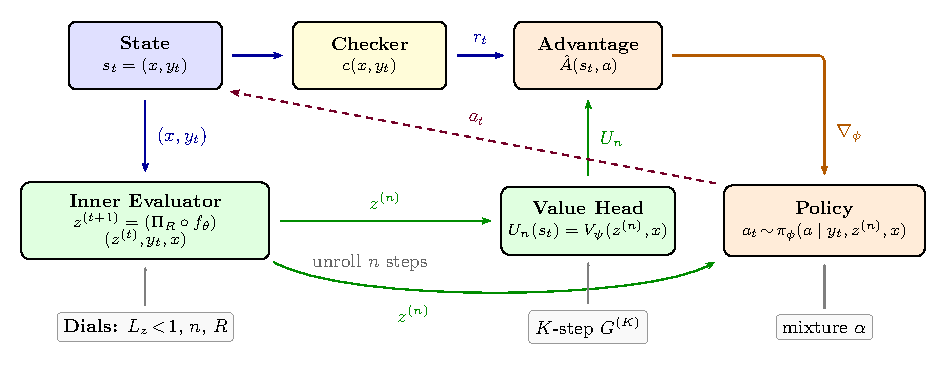
\includegraphics[width=0.72\columnwidth]{figures/diagram.pdf}
\caption{UPI--TRM architecture.
Solid arrows: data flow; dashed arrow: edit action $a_t$ updates plan $y_t \to y_{t+1}$.
The inner evaluator unrolls $n$ steps to produce latent $z^{(n)}$; the value head $V_\psi$ yields $U_n(s)$.
Checker reward $r_t$ and advantages $\hat A$ drive policy-gradient updates; the new policy is a conservative mixture $\pi_{\mathrm{new}}{=}(1{-}\alpha)\pi{+}\alpha\pi_{\mathrm{cand}}$.
\textbf{Legend:} \textit{blue} boxes = TRM evaluator dials ($L_z$, $n$, $R$); \textit{gray} boxes = standard algorithmic knobs ($K$, $\alpha$).}
\label{fig:rsi_architecture}
\end{figure}

\begin{table}[t]
\caption{TRM edit loop as plan-space MDP.
$f_\theta$: latent update network; $\Pi_R$: projection onto radius-$R$ ball; $V_\psi$: value head; $U_n(s)$: value after $n$ unrolls; $L_z\!<\!1$: contraction modulus; $s{=}(x,y)$: state; $\alpha$: mixture weight.
\textbf{Dials:} $L_z$, $n$. \textbf{Knobs:} $K$, $\alpha$.}
\label{table:overview}
\centering
\scriptsize
\setlength{\tabcolsep}{4pt}
\renewcommand{\arraystretch}{0.9}
\begin{tabular}{@{}lp{0.64\columnwidth}@{}}
\toprule
\multicolumn{2}{@{}l@{}}{\textbf{Inner evaluator (TRM)}} \\
\midrule
Latent unroll & $z^{(t+1)}\!=\!(\Pi_R\!\circ\!f_\theta)(z^{(t)},y,x)$ \\
Unrolled value & $U_n(s)=V_\psi(z^{(n)}(s),x)$ \\
Bias & Dial $L_z<1$; truncation error $\propto L_z^n$ \\
\midrule
\multicolumn{2}{@{}l@{}}{\textbf{Outer plan-space MDP}} \\
\midrule
State & $s=(x,y)$; instance $x$ fixed per episode \\
Action & $a\in\mathcal{A}(y)$; edit $y'=\mathrm{edit}(y,a;x)$ \\
Reward & Checker + shaping; discount $\gamma$ \\
Update & $\pi_{\mathrm{new}}=(1-\alpha)\pi+\alpha\pi_{\mathrm{cand}}$ \\
\bottomrule
\end{tabular}
\end{table}

\textbf{Contributions.}
\begin{enumerate}[nosep,leftmargin=*]
\item \textbf{Algorithm:} UPI--TRM, a policy-iteration template for TRMs trained from checker reward, combining $K$-step value regression, advantage-based improvement, and conservative mixture updates (\Cref{sec:algorithm}).
\item \textbf{Value decomposition:} Under inner-loop contraction ($L_z < 1$), we decompose value error into an architectural Bellman residual plus a truncation bias that decays as $L_z^{\,n}$ with unroll depth (Proposition~\ref{prop:error_bounds}).
\item \textbf{Conservative improvement:} For mixture updates with centered advantages, evaluation error enters the improvement bound scaled by the mixture weight~$\alpha$ rather than at full strength (Theorem~\ref{thm:monotone_with_error}); approximate centering degrades gracefully via a centering defect term.
\end{enumerate}

CPI (formalized in Section~\ref{sec:setup}) is the natural template here because the TRM evaluator is inherently approximate; our contribution is making the \emph{compute truncation} explicit, connecting TRM evaluator dials to CPI's safe-improvement thresholds.

\longonly{
\textbf{Positioning.}
Our plan-space MDP framing connects to learning-to-search~\citep{Daume2009SEARN,Ross2011DAgger,Chang2015LOLS} and RL with verifiable rewards, while our stability analysis builds on CPI and trust-region ideas~\citep{KakadeLangford2002,Schulman2015TRPO}.}

\section{Background and Setup}
\label{sec:setup}

\shortonly{
\textbf{Approximate and conservative policy iteration.}
Approximate policy iteration (API)~\citep{BertsekasTsitsiklis1996} alternates approximate evaluation and improvement; error propagation is governed by evaluation accuracy.
Conservative policy iteration (CPI)~\citep{KakadeLangford2002} restricts improvement to a mixture $\pi_{k+1} = (1{-}\alpha)\pi_k + \alpha\pi_{\mathrm{cand}}$, yielding the bound $\eta(\pi_{k+1}) \ge L_{\pi_k}(\pi_{k+1}) - \frac{2\gamma\varepsilon_{\mathrm{CPI}}}{(1-\gamma)^2}\alpha^2$ (where $L_{\pi_k}$ is the local surrogate).
This provides monotonic improvement that degrades gracefully with evaluation error, making CPI natural when the evaluator is approximate (as in TRMs with truncated unrolling).

\textbf{Notation.}
$s = (x, y)$ denotes a state (instance--plan pair); $z \in \mathbb{R}^d$ is the latent; $z^{(n)}$ is the latent after $n$ inner steps; $z^*$ is the fixed point. $L_z$ is the contraction modulus of the inner update; $L_V$ is the Lipschitz constant of the value head. $\varepsilon_{\mathrm{res}}^*$, $\varepsilon_A$, $\varepsilon_{A,\mathrm{cand}}$, $\varepsilon_{\mathrm{cent}}$ denote error quantities defined in Section~\ref{sec:error_bounds}.

We formalize plan editing as an MDP and introduce the TRM evaluator structure.

\textbf{Plan-space MDP.}
States $s=(x,y)$ pair an instance $x\in\XX$ (e.g., a puzzle) with a candidate plan $y\in\YY$.
Actions edit the plan: $y'=\mathrm{edit}(y,a;x)$.
A deterministic checker provides a bounded score $c(x,y)\in[0,C_{\max}]$.
We use potential-based shaping with potential $\Phi(s)=c(x,y)$, i.e.,
$r(s,a,s') = r_0(s,a,s') + \gamma \Phi(s') - \Phi(s)$,
where $r_0$ is nonzero only on transitions into the absorbing state $s_{\mathrm{abs}}$; we set $\Phi(s_{\mathrm{abs}})=C_{\max}$ so $V^\pi(s_{\mathrm{abs}})=-C_{\max}$ for all $\pi$ (constant shift; advantages unchanged).

\textbf{TRM evaluator.}
A Tiny Recursive Model maintains a latent $z\in\ZZ=\R^d$ updated via $z^{(t+1)}=f_\theta(z^{(t)},y,x)$.
After $n$ inner steps (with optional projection $\Pi_R$), we define the unrolled value as $U_n(s)=V_\psi(z^{(n)}(s),x)$.
The ideal (fixed-point) value is $U_*(s)=V_\psi(z^*(s),x)$ where $z^*$ is the unique fixed point of the $L_z$-contractive map $z\mapsto (\Pi_R\circ f_\theta)(z,y,x)$.

\textbf{Episodic-$z$ vs.\ persistent-$z$.}
Our primary analysis uses \emph{episodic-$z$}: the latent is reinitialized each edit step, giving Markov dynamics on $(x,y)$.
A persistent-$z$ extension (carrying $z$ across edits under a slow-drift assumption) is possible but not analyzed here.

\textbf{Advantage-evaluation closure.}
Conservative improvement requires value accuracy on on-policy states and one-step successors under candidate actions.
We write $\|\cdot\|_{\infty,\pi,\pi_{\mathrm{cand}}}^{\mathrm{adv}}$ for sup-norms over the closure $\mathcal{R}_{\pi,\pi_{\mathrm{cand}}}^{\mathrm{adv}} \supseteq \mathcal{R}_\pi$ that additionally contains these successors and is closed under $K$-step $\pi$-rollouts.
Under this closure, $\mathcal{T}^\pi_K$ is a $\gamma^K$-contraction.

\textbf{Key assumptions (used in bounds).}
\begin{assumption}[Bounded rewards]
\label{ass:bounded}
Shaped rewards satisfy $|r(s,a,s')|\le R_{\max}$ for all transitions.
\end{assumption}
\begin{assumption}[Bounded value head]
\label{ass:bounded_value_head}
There exists $V_{\max}<\infty$ such that $|V_\psi(z,x)| \le V_{\max}$ for all $z$ in the forward-invariant region $\mathcal{Z}_{\mathrm{inv}}$.
\end{assumption}
We assume the value head is $L_V$-Lipschitz in $z$:
\begin{equation}
\bigl|V_\psi(z,x)-V_\psi(z',x)\bigr| \le L_V\,\norm{z-z'}.
\label{eq:LV_def}
\end{equation}
\begin{proposition}[Fixed point and finite-unrolling bias]
\label{prop:banach}
Under Assumption~\ref{ass:Lip}, the projected recursion has a unique fixed point $z^*$, with $\|z^{(n)}-z^*\| \le \frac{L_z^n}{1-L_z}\,C_z$ where $C_z$ is as defined in Assumption~\ref{ass:Lip}.
\end{proposition}
}

\longonly{
We establish notation, define the plan-space MDP, and introduce key conventions that will be used throughout.

\textbf{Roadmap for the setup.}
Our analysis needs two simple technical devices beyond standard RL notation.
First, conservative improvement evaluates candidate actions from on-policy states, so to bound advantage error we require value accuracy not only on states visited by $\pi$ but also on their one-step successors under actions from $\pi$ and a candidate policy. This motivates the \emph{advantage-evaluation closure} in Definition~\ref{def:adv_closure}.
Second, because we use potential-based shaping, we explicitly fix a terminal boundary value (equivalently, a constant shift of the usual $V(s_{\mathrm{abs}})=0$ convention). This lets us write $K$-step operators without special-casing early termination while keeping advantages and policy improvement unchanged.

\subsection{Notation and Conventions}
\label{sec:notation}

We use $\|\cdot\|_\infty$ for sup-norms over state spaces and $$\|\cdot\| \coloneqq \|\cdot\|_2$$ for the Euclidean norm on the latent space $\ZZ=\R^d$.
All Lipschitz constants ($L_z$, $L_V$, etc.) and the projection $\Pi_R$ are taken with respect to this Euclidean norm.
We work in the Banach space of bounded real-valued functions equipped with $\|\cdot\|_\infty$.
When we need to emphasize the domain of a sup-norm, we write $\supnorm{f}{\Pi}$ for the sup-norm over the reachable set $\mathcal{R}_\Pi$ (defined below).
}

\longonly{
\begin{table}[t]
\caption{Summary of key notation.}
\label{tab:notation_key}
\centering
\scriptsize
\begin{tabular}{@{}ll@{}}
\toprule
Symbol & Meaning \\
\midrule
$\XX, \YY, \ZZ$ & Input, plan, latent spaces \\
$\SSS_{\mathrm{plan}}$ & Plan-space state (episodic-$z$) \\
$\tilde{\SSS}$ & Persistent-$z$ state space \\
$s\!=\!(x,y)$, $\tilde s\!=\!(x,y,z)$ & Plan-space states \\
$s_{\mathrm{abs}}$ & Absorbing terminal state \\
$\mathcal{Z}_{\mathrm{inv}}$ & Forward-invariant region \\
$f_\theta$, $\tilde f_\theta$ & Recursion map, projected map \\
$z^*(x,y)$ & Fixed point \\
$V_\psi(z,x)$ & Latent value head \\
$L_z \!\in\! (0,1)$ & Contraction modulus \\
$C_z$, $R$ & First-update bound, projection radius \\
$L_V$ & Lipschitz constant of $V_\psi$ \\
$\Cdrift(n)$ & Drift constant (persistent-$z$) \\
$\|\cdot\|_{\infty,\Pi}$ & Sup-norm over $\mathcal{R}_\Pi$ \\
\bottomrule
\end{tabular}
\end{table}}

\longonly{
\begin{definition}[Reachable set]
\label{def:reachable}
For a policy $\pi$, let $\mathcal{R}_\pi$ be the set of states $s$ such that
$\Pr_\pi(\exists\, t\ge 0:\; s_t=s \mid s_0\sim\rho)>0$. Let $\rho$ denote a fixed initial-state distribution over $\SSS_{\mathrm{plan}}$ (defined in \Cref{sec:meta_mdp}).

\emph{Convention (absorbing state).}
We include the absorbing terminal state $s_{\mathrm{abs}}$ in function domains purely for closure under transitions during $K$-step rollouts.
We set the boundary value exactly, so Bellman residuals and value errors at $s_{\mathrm{abs}}$ are identically zero: including or excluding $s_{\mathrm{abs}}$ from sup-norms does not change any bound.
Readers who prefer the standard $V(s_{\mathrm{abs}})=0$ convention can shift the shaping potential by a constant; this leaves advantages and policy improvement unchanged.
\end{definition}

\begin{definition}[Advantage-evaluation closure]
\label{def:adv_closure}
Fix a current policy $\pi$ and a candidate policy $\pi_{\mathrm{cand}}$.
Let $\mathcal{R}_{\pi,\pi_{\mathrm{cand}}}^{\mathrm{adv}}$ be any state set that contains $\mathcal{R}_\pi$ and all one-step successors of states in $\mathcal{R}_\pi$ obtained by actions in $\mathrm{supp}(\pi(\cdot|s))\cup\mathrm{supp}(\pi_{\mathrm{cand}}(\cdot|s))$. We further require that $\mathcal{R}_{\pi,\pi_{\mathrm{cand}}}^{\mathrm{adv}}$ is closed under forward dynamics of $\pi$.
Concretely, $\mathcal{R}_{\pi,\pi_{\mathrm{cand}}}^{\mathrm{adv}}$ includes all states reachable within $K+1$ steps from initial states under any mixture of $\pi$ and $\pi_{\mathrm{cand}}$.
We write $\|f\|_{\infty,\pi,\pi_{\mathrm{cand}}}^{\mathrm{adv}} := \sup_{s\in \mathcal{R}_{\pi,\pi_{\mathrm{cand}}}^{\mathrm{adv}}} |f(s)|$.
As with $\mathcal{R}_\pi$, all norms implicitly include $s_{\mathrm{abs}}$: $\|f\|_{\infty,\pi,\pi_{\mathrm{cand}}}^{\mathrm{adv}} = \sup_{s\in \mathcal{R}_{\pi,\pi_{\mathrm{cand}}}^{\mathrm{adv}}\cup\{s_{\mathrm{abs}}\}} |f(s)|$.
\end{definition}

\textbf{Standard RL quantities.}
We adopt standard discounted MDP notation~\citep{SuttonBarto2018,Puterman1994}.
For any policy $\pi$, the value function is
$V^\pi(s)=\E_\pi[\sum_{t\ge0}\gamma^t r(s_t,a_t,s_{t+1}) \mid s_0=s]$,
the action-value function is
$Q^\pi(s,a)=\E_\pi[r(s,a,s_1)+\sum_{t\ge1}\gamma^t r(s_t,a_t,s_{t+1}) \mid s_0=s,a_0=a]$,
and the advantage is $A^\pi(s,a)=Q^\pi(s,a)-V^\pi(s)$, satisfying $\E_{a\sim\pi(\cdot|s)}[A^\pi(s,a)]=0$.

\subsection{Tiny Recursive Models}
\label{sec:trm_brief}

We consider tasks with inputs $x\in\XX$ and structured outputs $y\in\YY$ (grids, sequences, or symbolic structures).
TRM maintains
(i)~an internal latent reasoning state $z\in\ZZ$;
(ii)~a plan $y$; and
(iii)~a small update network $f_\theta:\ZZ\times\YY\times\XX\to\ZZ$.
On each inner step $t$, the latent reasoning state is updated via
\begin{equation}
    z^{(t+1)} = f_\theta\bigl(z^{(t)},y,x\bigr),
    \qquad
    t = 0,1,\dots.
    \label{eq:inner}
\end{equation}
After $n$ inner steps, an edit policy modifies the plan using $z^{(n)}$ and input $x$.



We introduce a parametric edit policy $\pi_\phi(a\mid y,z,x)$ over edit actions $a$, and a deterministic edit operator $y' = \mathrm{edit}(y,a;x)$. This makes the outer edit loop an explicit decision process, allowing us to (i) train the edit policy directly from checker rewards, and (ii) analyze the stability of policy updates as a function of evaluator design and compute (the unrolling depth $n$).

\textbf{Relation to the original TRM edit rule.}
In the original TRM pseudocode, the model repeatedly refines its answer while updating latent features, and training uses deep supervision with an early-stopping signal~\citep{TRM2025}.
Our formulation separates \emph{evaluation} (the $n$-step latent unroll producing $z^{(n)}$) from \emph{editing} (an explicit policy $\pi_\phi$ over plan edits).
This separation is convenient for reinforcement learning from checker rewards: the environment state is the current plan, while the evaluator is a compute-truncated internal dynamical system.

\longonly{
\begin{remark}[Mapping to original TRM]
\label{rem:trm_mapping}
In the original TRM implementation~\citep{TRM2025}: (i) the latent $z$ is persistent across edit steps (our persistent-$z$ variant); (ii) deep supervision provides intermediate targets during training; (iii) an ACT-style halting head determines when to stop inner iterations.
Our episodic-$z$ variant simplifies analysis by reinitializing $z$ each step, yielding Markov dynamics on $\SSS_{\mathrm{plan}}$.
Our RL formulation replaces deep supervision with checker-based rewards.
\end{remark}}

\subsection{Plan-space MDP}
\label{sec:meta_mdp}
We formalize a plan-space MDP over instance--plan pairs $(x,y)$, which is closely related to ``learning to search'' and structured prediction as sequential decision making~\citep{Daume2009SEARN,Ross2011DAgger,Chang2015LOLS}, but uses checker rewards rather than expert demonstrations.
This is an ordinary discounted MDP over $\SSS_{\mathrm{plan}}=\XX\times\YY$; we do not rely on any meta-learning structure.

\textbf{State space and absorbing state.}
We draw an instance $x \sim \mathcal{D}$ and an initial plan $y_0 \sim \iota(\cdot \mid x)$, which together induce the initial-state distribution $\rho(x,y_0)=\mathcal{D}(x)\,\iota(y_0\mid x)$.
Here $\mathcal{D}$ denotes the task/data distribution over inputs (e.g., a dataset of Sudoku puzzles), and $\iota(\cdot \mid x)$ is the initialization distribution over plans given instance $x$ (e.g., in Sudoku we take $y_0=x$, the plan initially equals the clue grid, or $y_0$ is the empty grid with clues filled).
We augment $\SSS_{\mathrm{plan}}$ with an absorbing terminal state $s_{\mathrm{abs}}$ representing solved episodes or termination.
Once $s_t=s_{\mathrm{abs}}$, we have $s_{t+k}=s_{\mathrm{abs}}$ for all $k\ge 1$ (i.e., $P(s_{\mathrm{abs}}\mid s_{\mathrm{abs}},a)=1$ for all $a$).

\textbf{Rewards (checker + potential shaping).}
A task-specific checker provides a bounded score $c(x,y)\in[0,C_{\max}]$.
Transitions are deterministic: $y'=\mathrm{edit}(y,a;x)$.
\begin{remark}[Stochasticity]
For clarity we present deterministic edits and a deterministic checker, as in Sudoku.
Our analysis extends to stochastic transitions and noisy checkers by interpreting $r(s,a,s')$ and Bellman operators under the usual expectation over $P(\cdot\mid s,a)$.
\end{remark}


We use potential-based shaping with $\Phi(x,y)=c(x,y)$:
\begin{equation}
r(s,a,s') = r_0(s,a,s') + \gamma \Phi(s') - \Phi(s),
\label{eq:shaping}
\end{equation}
where base reward $r_0$ is nonzero only on transitions entering the absorbing state.
This preserves optimal policies~\citep{Ng1999Shaping}.
We adopt an absorbing-state normalization with $V^\pi(s_{\mathrm{abs}})=-C_{\max}$ for all $\pi$.

\begin{assumption}[Bounded rewards]
\label{ass:bounded}
We use potential-based shaping~\eqref{eq:shaping}, yielding a \emph{shaped reward} $r(s,a,s')$.
We assume these shaped rewards are uniformly bounded: $|r(s,a,s')|\le R_{\max}$ for all transitions.

%Shaped  rewards are uniformly bounded: $|r(s,a,s')|\le R_{\max}$ for all transitions (including the absorbing self-loop).
Consequently, by the geometric series bound $|\sum_{t\ge 0} \gamma^t r_t| \le \sum_{t\ge 0} \gamma^t R_{\max} = R_{\max}/(1-\gamma)$, for any policy $\pi$ we have
$|V^\pi(s)|\le \frac{R_{\max}}{1-\gamma}$ and $|A^\pi(s,a)|\le \frac{2R_{\max}}{1-\gamma}$~\citep[Ch.~3]{Puterman1994}.
\end{assumption}

Consequently, for any policy $\pi$ and any state $s$ (including $s_{\mathrm{abs}}$),
the discounted return is uniformly bounded:
\begin{equation}
\begin{aligned}
|V^\pi(s)| &\le \frac{R_{\max}}{1-\gamma}, \\
\sup_{a} |Q^\pi(s,a)| &\le \frac{R_{\max}}{1-\gamma}, \\
\sup_{a} |A^\pi(s,a)| &\le \frac{2R_{\max}}{1-\gamma}.
\end{aligned}
\label{eq:value_adv_bounds_from_Rmax}
\end{equation}
In particular, the CPI constant satisfies
$\varepsilon_{\mathrm{CPI}}=\max_s\bigl|\E_{a\sim\pi_{\mathrm{cand}}(\cdot|s)}A^\pi(s,a)\bigr|
\le 2R_{\max}/(1-\gamma)$.

\textbf{Discounted occupancy and performance.}
We fix discount $\gamma\in[0,1)$. The case $\gamma=0$ is degenerate (a one-step greedy objective) but allowed; all bounds hold and simplify. The interesting regime for multi-step plan editing is $\gamma\approx 1$.
A policy $\pi(a\mid s)$ induces the normalized discounted occupancy:
\begin{equation}
    d_\pi(s)
    =
    (1-\gamma)
    \sum_{t\ge 0}
    \gamma^t \Pr(s_t = s \mid s_0\sim\rho,\pi).
\end{equation}
This definition makes $d_\pi$ a probability distribution, as factor $(1-\gamma)$ normalizes the discounted visitation counts.
Using the standard occupancy-measure identity, a direct rearrangement of the discounted return gives
\begin{align}
\eta(\pi)
&=
\E_{s_0\sim\rho}\bigl[V^\pi(s_0)\bigr]
\notag\\
&=
\frac{1}{1-\gamma}\,
\E_{\substack{s\sim d_\pi,\, a\sim\pi(\cdot\mid s) \\ s'\sim P(\cdot\mid s,a)}}[r(s,a,s')];
\end{align}
see~\citet{KakadeLangford2002,Puterman1994}.

\subsection{Episodic-$z$ vs.\ persistent-$z$ variants}
\label{sec:reset_persistent}

The inner evaluator maintains a latent state $z$.
A key design choice is whether $z$ is reinitialized at each edit step or carried across steps:
\begin{itemize}
\item \textbf{Episodic-$z$ (primary setting):} The latent is reinitialized to $z_{\mathrm{init}}(x,y_t)$ at each edit step $t$.
The MDP state is $s=(x,y)\in\SSS_{\mathrm{plan}}=\XX\times\YY$, yielding Markov dynamics.
This variant admits cleaner analysis and is our main focus.
\item \textbf{Persistent-$z$:} The latent is carried across edits: the state is $\tilde s=(x,y,z)\in\tilde{\SSS}=\XX\times\YY\times\ZZ$.
This matches the original TRM architecture but complicates analysis because the latent's fixed point drifts as $y$ changes.
Extensions under a slow-drift condition are possible but omitted for space.
\end{itemize}

\longonly{
\begin{table}[t]
\caption{Comparison of episodic-$z$ and persistent-$z$ variants.}
\label{tab:variants}
\centering
\scriptsize
\resizebox{\linewidth}{!}{%
\begin{tabular}{@{}lll@{}}
\toprule
Property & Episodic-$z$ & Persistent-$z$ \\
\midrule
State space & $\SSS_{\mathrm{plan}} = \XX \times \YY$ & $\tilde{\SSS} = \XX \times \YY \times \ZZ$ \\
Latent init & $z^{(0)} = z_{\mathrm{init}}(x,y)$ & Carried: $z_0 \to z_1 \to \cdots$ \\
Markov? & Yes (in $(x,y)$) & Yes (in $(x,y,z)$) \\
Theory & Primary (simpler) & Via slow-drift \\
TRM match & Simplified & Original architecture \\
\bottomrule
\end{tabular}%
}
\end{table}
}

\subsection{TRM as unrolled generalized policy iteration}
\label{sec:gpi_view}

We attach a value head $V_\psi:\ZZ\times\XX\to\R$ on top of the latent.
In the episodic-$z$ setting, for $s=(x,y)$ we define
\begin{equation}
    z^{(n)}(s)
    =
    (\Pi_R \circ f_\theta)^{\circ n}\bigl(z_{\mathrm{init}}(x,y),y,x\bigr).
\end{equation}
Here $\Pi_R$ is the projection defined in~\eqref{eq:projection} and is applied at \emph{each} inner step to ensure forward-invariance:
\begin{equation}
\begin{split}
\Pi_R(z) &= \arg\min_{u:\|u\|_2\le R}\|u-z\|_2 \\
&=
\begin{cases}
z, & \|z\|_2 \le R,\\[2pt]
R\,\dfrac{z}{\|z\|_2}, & \|z\|_2 > R.
\end{cases}
\end{split}
\label{eq:projection}
\end{equation}
In particular, $\Pi_R(0)=0$.
If the projection is disabled, take $\Pi_R$ to be the identity map.

\noindent\emph{Convention (projection off).} Equation~\eqref{eq:projection} defines Euclidean projection for $R>0$; when projection is disabled we set $\Pi_R$ to the identity map (in experiments we denote this configuration by ``$R{=}0$ / proj.\ off'' as a sentinel, not as projection onto a radius-$0$ ball).

\emph{Interior projection fixed points.}
If a fixed point $z^*$ of the projected map $\tilde f_\theta = \Pi_R \circ f_\theta$ lies strictly inside the ball ($\|z^*\|_2 < R$), then the projection is inactive and $z^*$ also satisfies the unprojected fixed-point equation $f_\theta(z^*,y,x) = z^*$.
This follows from continuity: if $\|z^*\|_2 < R$, then $\Pi_R(z) = z$ in a neighborhood of $z^*$, so $f_\theta(z^*,y,x) = \tilde f_\theta(z^*,y,x) = z^*$.

\begin{remark}[Latent projection vs.\ projected TD]
\label{rem:projection_distinction}
Our projection $\Pi_R$ is a \emph{latent-space Euclidean projection} applied inside the evaluator recursion to enforce forward-invariance of iterates $z^{(t)}$.
This is fundamentally different from the \emph{projected Bellman operator} in function-approximation TD, which projects value functions onto a function class and can cause divergence~\citep{Baird1995Residual,TsitsiklisVanRoy1997}.
Under the Euclidean norm, $\Pi_R$ is non-expansive (1-Lipschitz): if $f_\theta$ is $L_z$-Lipschitz in $z$, then $\Pi_R\circ f_\theta$ remains $L_z$-Lipschitz.
The latent projection preserves contraction and does not introduce the divergence risks associated with projected TD.
Our analysis concerns error propagation in evaluation$\rightarrow$improvement steps, not the learning dynamics of TD itself.
\end{remark}

The \emph{unrolled value} is defined as
\begin{equation}
    U_n(s)
    \triangleq
    V_\psi\bigl(z^{(n)}(s),x\bigr).
    \label{eq:Un_def}
\end{equation}
If the inner recursion (with per-step projection) were run to convergence, it would reach the unique fixed point
$z^*(x,y)$ of the \emph{actual per-step update map} $\tilde f_\theta(\cdot,y,x) := (\Pi_R\circ f_\theta)(\cdot,y,x)$.
If the fixed point lies strictly inside the projection ball ($\|z^*(x,y)\|_2 < R$), then projection is locally inactive and $z^*$ also satisfies the unprojected fixed-point equation $f_\theta(z^*,y,x)=z^*$ (Lemma~\ref{lem:interior_proj}).
The corresponding \emph{ideal latent value} is:
\begin{equation}
    U_*(s) = V_\psi\bigl(z^*(s),x\bigr).
    \label{eq:Ustar_def}
\end{equation}

\textbf{Absorbing-state extension.}
The definitions~\eqref{eq:Un_def} and~\eqref{eq:Ustar_def} apply to plan-space states $s=(x,y)\in\SSS_{\mathrm{plan}}$.
For consistency with sup-norms over $\SSS_{\mathrm{plan}}\cup\{s_{\mathrm{abs}}\}$, we extend both functions to the absorbing state:
\begin{equation}
U_n(s_{\mathrm{abs}}) := -C_{\max}, \qquad U_*(s_{\mathrm{abs}}) := -C_{\max}.
\label{eq:U_sabs_extension}
\end{equation}
This is consistent with the shaping convention $V^\pi(s_{\mathrm{abs}})=-C_{\max}$ for all $\pi$.
Throughout, sup-norms in Bellman operators are taken over $\mathcal{R}_\pi \cup \{s_{\mathrm{abs}}\}$ (or $\mathcal{R}_{\pi,\pi_{\mathrm{cand}}}^{\mathrm{adv}} \cup \{s_{\mathrm{abs}}\}$ for advantages).

\longonly{
\begin{sloppypar}
\begin{remark}[Conceptual vs.\ computable quantities]
\label{rem:conceptual}
$U_*$ equals $V^\pi$ only if $(f_\theta, V_\psi)$ exactly matches the true value function; in general $\|U_* - V^\pi\|_\infty$ is an architectural approximation error.
The quantity $U_*$ is a \emph{conceptual tool} for separating approximation error from unrolling bias---we cannot compute it directly.
In practice, one monitors the empirical $K$-step residual of $U_n$ as a proxy: if the residual is small and $n$ is large (so $\|U_n - U_*\|$ is small by Proposition~\ref{prop:banach}), Lemma~\ref{lem:residual_transfer} implies the architectural residual is also small.
\end{remark}

The resulting picture is generalized policy iteration in plan-space: train $(f_\theta,V_\psi)$ so $U_n\approx V^\pi$, then update $\pi_\phi$ via advantages.
\end{sloppypar}
}% end of longonly for conceptual remark
}% end of longonly for detailed Section 2

\shortonly{
\section{Algorithm Sketch}
\label{sec:algorithm}
We alternate three phases: (i)~$K$-step bootstrapped value regression for $U_n$, (ii)~a policy improvement step producing a candidate $\pi_{\mathrm{cand}}$, and (iii)~a conservative mixture update $\pi_{\mathrm{new}}\!=\!(1{-}\alpha)\pi+\alpha\pi_{\mathrm{cand}}$ (with optional distillation).

\textbf{Phase 1: Value regression.}
We form $K$-step rollouts and define a target with target network $V_{\bar\psi}$:
\begin{equation}
G^{(K)}(s_0)
=
\sum_{k=0}^{K-1}\gamma^k r_k
+
\gamma^K \bar V(s_K).
\label{eq:GK_def}
\end{equation}
where $\bar V(s):=-C_{\max}$ if $s=s_{\mathrm{abs}}$, and otherwise $\bar V(s)=V_{\bar\psi}(z^{(n)}(s),x)$.
We minimize the bootstrapped value loss
$\mathcal{L}_{\mathrm{val}}(\psi,\theta)
=
\E_{s_0\sim\mu}\bigl[
   (V_\psi(z^{(n)}(s_0),x_0)
   -
   \sg(G^{(K)}(s_0)))^2
\bigr]$.

\textbf{Phase 2: Advantage estimation.}
We define $\widehat Q_V(s,a) = \E_{s'}[r(s,a,s') + \gamma V(s')]$ and the centered advantage $\widehat A_V(s,a) = \widehat Q_V(s,a) - B_V(s)$, where $B_V(s)=\E_{b\sim\pi}[\widehat Q_V(s,b)]$ yields exact statewise centering (Theorem~\ref{thm:monotone_with_error}).

\textbf{Phase 3: Conservative update.}
Form the candidate $\pi_{\mathrm{cand}}$ via policy gradient on $\widehat A$, then mix:
$\pi_{\mathrm{new}}=(1-\alpha)\pi+\alpha\pi_{\mathrm{cand}}$.
Distill back to a single network: $\pi_\phi \gets \arg\min_\phi \KL(\pi_{\mathrm{new}} \| \pi_\phi)$.

\begin{remark}[Theory--implementation gap]
\label{rem:distillation_penalty}
Theorem~\ref{thm:monotone_with_error} applies to the explicit mixture $\pi_{\mathrm{new}}{=}(1{-}\alpha)\pi{+}\alpha\pi_{\mathrm{cand}}$, not to the distilled policy $\pi_\phi$.
Distillation introduces approximation error not covered by our bounds.
In experiments $\KL(\pi_{\mathrm{new}}\|\pi_\phi)$ stays below $10^{-3}$; by Pinsker's inequality, per-state TV distance is below $0.03$.
The bounds should be read as structural guidance for how $(L_z, n, \alpha)$ affect safe improvement, not as an end-to-end certificate for the implemented algorithm.
\end{remark}

\textbf{Dials and knobs.}
Our bounds expose two TRM evaluator dials---$L_z$ (contraction modulus) and $n$ (unroll depth)---controlling truncation bias, and two standard algorithmic knobs---$K$ (bootstrap horizon) and $\alpha$ (mixture weight)---controlling residual amplification and conservativeness.

The theory in Sections~\ref{sec:contraction}--\ref{sec:cpi} analyzes a single evaluation$\rightarrow$improvement step of this template under idealized assumptions.}

\longonly{
\section{Algorithmic Template: UPI--TRM}
\label{sec:algorithm}

\textbf{Algorithm presentation note.}
Our main theoretical results (Sections~\ref{sec:value_error_bounds}--\ref{sec:cpi}) analyze the \emph{episodic-$z$} variant, where the latent $z$ is reinitialized at each edit step.
\Cref{alg:upi} is presented in the \emph{persistent-$z$} form (carrying $z$ across steps) because it matches the original TRM design.
Remark~\ref{rem:episodic_z_algo} clarifies the episodic-$z$ special case.
Corollary~\ref{cor:persistent_value_adv} extends bounds to persistent-$z$ under a slow-drift assumption.

\begin{algorithm}[t]
\small
\caption{UPI--TRM: single interaction + update step}
\label{alg:upi}
\begin{algorithmic}[1]
\STATE \textbf{Input:} $x, y_0, z_0, \gamma, n, K, \alpha, \tau, R$
\STATE Initialize $\tilde{s}_0 \gets (x,y_0,z_0)$; $\mathit{done} \gets \mathrm{false}$
\FOR{$k = 0$ to $K-1$}
  \IF{$\mathit{done}$}
    \STATE $r_k \gets (\gamma-1)C_{\max}$; $\tilde{s}_{k+1} \gets s_{\mathrm{abs}}$ \hfill \emph{// Absorbing self-loop}
  \ELSE
    \STATE $z_k^{(n)} \gets (\Pi_R \circ f_\theta)^{\circ n}(z_k,y_k,x)$ \hfill \emph{// $n$ inner steps}
    \STATE Sample $a_k \sim \pi_{\phi}(a \mid y_k,z_k^{(n)},x)$
    \STATE $y_{k+1} \gets \mathrm{edit}(y_k,a_k;x)$; receive $r_k$
    \STATE $z_{k+1} \gets z_k^{(n)}$ \hfill \emph{// Persistent-z variant (carry latent)}
    \STATE \emph{// For Episodic-z (theory), use: } $z_{k+1} \gets z_{\mathrm{init}}(x,y_{k+1})$
    \STATE $\tilde{s}_{k+1} \gets (x,y_{k+1},z_{k+1})$
    \IF{terminated}
     \STATE $\mathit{done} \gets \mathrm{true}$; $\tilde{s}_{k+1} \gets s_{\mathrm{abs}}$
    \ENDIF
  \ENDIF
\ENDFOR
\STATE Compute target $G^{(K)}$ via~\eqref{eq:GK_def}
\STATE Update $(\theta,\psi)$ by minimizing $\mathcal{L}_{\mathrm{val}}$~\eqref{eq:KBR_loss}
\STATE Form advantages $\widehat A$\longonly{ via~\eqref{eq:Ahat_def}}\shortonly{ via centered one-step estimate}
\STATE Policy gradient step $\to$ candidate $\pi_{\mathrm{cand}}$
\STATE $\pi_{\mathrm{new}} \gets (1-\alpha)\pi_{\phi} + \alpha\pi_{\mathrm{cand}}$
\STATE Distill: $\pi_\phi \gets \arg\min_\phi \KL(\pi_{\mathrm{new}} \| \pi_\phi)$
\STATE $\bar\psi \gets \tau \bar\psi + (1-\tau)\psi$
\end{algorithmic}
\end{algorithm}

The theory in Sections~\ref{sec:bellman}--\ref{sec:cpi} analyzes a single evaluation--improvement step of this template under idealized assumptions.

\begin{remark}[Episodic-$z$ special case]
\label{rem:episodic_z_algo}
In the episodic-$z$ variant, we skip the ``carry latent'' step (line 10). Instead, at the start of each loop iteration, we reinitialize $z_k \gets z_{\mathrm{init}}(x,y_k)$.
Our theoretical bounds in Sections~\ref{sec:value_error_bounds}--\ref{sec:cpi} apply directly; Corollary~\ref{cor:persistent_value_adv} extends to the persistent-$z$ case.
\end{remark}

\begin{remark}[Mapping dials to algorithm]
Table~\ref{tab:dial_mapping} connects the theoretical dials to Algorithm~\ref{alg:upi} parameters.
Lines 1--19 correspond to the theoretical GPI-with-mixture setting; the distillation in line 20 is essential for updating $\phi$ but lies outside our formal guarantee.
Practitioners can evaluate with the true mixture $\pi_{\mathrm{new}}$ (no distillation) if strict guarantees are needed, treating distillation as optional compression.
\end{remark}

\begin{table}[t]
\caption{Mapping dials to algorithm and theory.}
\label{tab:dial_mapping}
\centering
\small
\begin{tabular*}{\columnwidth}{@{\extracolsep{\fill}}lll@{}}
\toprule
Dial & Algorithm Line & Theorem \\
\midrule
$n$ (inner steps) & Line 7 & Prop.~\ref{prop:banach}\longonly{, Cor.~\ref{cor:epsA_dials}} \\
$K$ (horizon) & Line 3 loop & Prop.~\ref{prop:error_bounds} \\
$\alpha$ (mixture) & Line 19 & Thm.~\ref{thm:monotone_with_error} \\
$L_z$ (contraction) & Norm clamp & Assump.~\ref{ass:Lip} \\
$R$ (projection) & Line 7 & Def.~\ref{def:forward_invariant} \\
\bottomrule
\end{tabular*}
\end{table}

\subsection{Practical Details}
\label{sec:practical}

In practice we use replay buffers and mini-batches.
For advantage estimation we use either
(i)~the centered estimator\longonly{~\eqref{eq:Ahat_def}} $\widehat A = \widehat Q - B_V$ with an \emph{exactly computed} baseline $B_V(s)=\E_{b\sim\pi}[\widehat Q_V(s,b)]$ (tractable for discrete actions), preserving statewise centering $\E_{a\sim\pi}[\widehat A(s,a)]=0$---the regime of Theorem~\ref{thm:monotone_with_error} with $O(\alpha\varepsilon_{A,\mathrm{cand}})$ penalty---or
(ii)~a GAE-style estimator, where centering holds approximately and the guarantee degrades via $\varepsilon_{\mathrm{cent}}$ (Remark~\ref{rem:approx_centering}).

We also use:
norm control on $z{\to}z$ pathways (operator-norm clamping, per-layer scaling) to target $L_z<1$;
optional $z{\to}V$ norm control to bound~$L_V$;
explicit projection~\eqref{eq:projection} for forward-invariance;
empirical monitoring of $\hat L_z$, $\hat C_z$, $\widehat{L}_{z^*}$;
and distillation to update the policy network.

We log empirical proxies for the theoretical quantities ($\hat L_z$, $\hat C_z$, residuals, KL divergence).

The horizon $K$ trades bias against variance: larger $K$ shrinks the coefficient $(1-\gamma^K)^{-1}$ (tightening the bound \emph{for a fixed/comparable $K$-step residual}) but can change the $K$-step residual itself and increases target variance.
The mixture coefficient $\alpha$ or TRPO-style KL trust-region size should be chosen conservatively relative to estimated evaluation error.
Adaptive schemes that increase $\alpha$ when empirical TD errors are small can accelerate learning while maintaining safety.

\textbf{Exact baseline for discrete actions.}
For Sudoku-style tasks with discrete edits (e.g., ``set cell $(i,j)$ to~$d$''), exact baseline summation is feasible.
For larger spaces, use action-value estimation or sampling-based baselines.}

\section{Stability via Contraction of the Inner Evaluator}
\label{sec:contraction}

\shortonly{
% Compressed Bellman section for ICML short version
The Bellman operator $\mathcal{T}^\pi$ and its $K$-step version $\mathcal{T}^\pi_K$ are standard~\citep{SuttonBarto2018,Puterman1994}:
\begin{equation}
(\mathcal{T}^\pi_K V)(s) \;:=\; \E_\pi\!\Bigl[\textstyle\sum_{t=0}^{K-1}\gamma^t r_t + \gamma^K V(s_K)\,\Big|\,s_0=s\Bigr].
\label{eq:TK_def_short}
\end{equation}
The $K$-step operator is a $\gamma^K$-contraction with unique fixed point $V^\pi$.
We train the unrolled value $U_n$ by $K$-step bootstrapped regression, minimizing $\mathcal{L}_{\mathrm{val}}(\psi,\theta)=\E_{s_0\sim\mu}[(V_\psi(z^{(n)}(s_0),x_0)-\mathrm{sg}(G^{(K)}(s_0)))^2]$ with $G^{(K)}$ as defined in~\eqref{eq:GK_def}.
We do not derive a general $L^2(\mu)\to\|\cdot\|_\infty$ conversion; our bounds should be read as conditional on controlling the sup-norm residuals over the relevant closure set.}

\longonly{
We now introduce the Bellman operators that underpin our value-error analysis. The definitions below are standard~\citep{SuttonBarto2018,Puterman1994}; our novelty lies in connecting these operators to the inner-loop contraction structure of TRM.

For a fixed edit policy $\pi$, the Bellman operator is
\begin{align}
   (\mathcal{T}^\pi V)(s)
   &=
   \E_{a\sim\pi(\cdot\mid s),\, s'\sim P(\cdot\mid s,a)}\Big[
      r(s,a,s') + \gamma V(s')
   \Big].
   \label{eq:Bellman_operator}
\end{align}
Note that $r$ here includes the potential-based shaping term from~\eqref{eq:shaping}.
The $K$-step operator is $\mathcal{T}^\pi_K = (\mathcal{T}^\pi)^K$:
\begin{equation}
 (\mathcal{T}^\pi_K V)(s)
 =
 \E\Biggl[
   \sum_{k=0}^{K-1}\gamma^k r_k
   + \gamma^K V(s_K)
 \Biggr].
 \label{eq:K_step_T}
\end{equation}
Note that $K=1$ recovers the usual one-step Bellman operator.

\begin{lemma}[Contraction of $\mathcal{T}^\pi_K$ (textbook)]
\label{lem:Kstep_contraction}
For $\gamma\in(0,1)$ and $K\ge 1$,
$\|\mathcal{T}^\pi_K V-\mathcal{T}^\pi_K W\|_\infty \le \gamma^K \|V-W\|_\infty$,
where $\|\cdot\|_\infty$ is taken over any state set closed under forward dynamics of $\pi$ containing $s_{\mathrm{abs}}$.
The unique fixed point is $V^\pi$.
\end{lemma}
\emph{This is standard~\citep{Denardo1967,Puterman1994}; the $K$-step operator $\mathcal{T}^\pi_K$ is a $\gamma^K$-contraction, so for any bounded $\bar V$, $\|\mathcal{T}^\pi_K \bar V - V^\pi\|_\infty \le \gamma^K \|\bar V - V^\pi\|_\infty$ and iterating gives the resolvent bound.}
We include the absorbing state $s_{\mathrm{abs}}$ in the domain of the operator.
Under our shaping convention (shaping applied on all transitions), the absorbing self-loop reward is
$r(s_{\mathrm{abs}},a,s_{\mathrm{abs}})=(\gamma-1)C_{\max}$, which implies the fixed boundary value
$V^\pi(s_{\mathrm{abs}})=-C_{\max}$ for every policy $\pi$.
By Definition~\ref{def:reachable}, $\mathcal{R}_\pi$ is closed under transitions, so states reached during $K$-step rollouts remain in the domain and the contraction property holds on $\mathcal{R}_\pi\cup\{s_{\mathrm{abs}}\}$.

\subsection{Bootstrapped $K$-step training}
\label{sec:bootstrapped_training}

Given policy $\pi_\phi$, we train $(f_\theta,V_\psi)$ so that $U_n$ approximates $V^\pi$.
We form $K$-step rollouts and define a target with target network $V_{\bar\psi}$:
\begin{equation}
G^{(K)}(s_0)
=
\sum_{k=0}^{K-1}\gamma^k r_k
+
\gamma^K \, \bar V(s_K),
\label{eq:GK_def}
\end{equation}
where we define the bootstrap as
\[
\bar V(s)
=
\begin{cases}
V_{\bar\psi}\bigl(z^{(n)}(s),x\bigr), & s=(x,y)\in\SSS_{\mathrm{plan}},\\
-C_{\max}, & s=s_{\mathrm{abs}}.
\end{cases}
\]

\emph{Why $-C_{\max}$?}
Because we apply potential-based shaping on \emph{all} transitions including the absorbing self-loop, the shaped self-loop reward becomes $(\gamma-1)C_{\max}$, which implies the fixed boundary value $V^\pi(s_{\mathrm{abs}})=-C_{\max}$ for every policy.
This differs from the standard $V(s_{\mathrm{abs}})=0$ convention only by a constant shift of the potential, which leaves advantages and optimal policies unchanged.


\textbf{Termination convention.}
Rollouts are treated as always having length $K$ in the augmented MDP: if $s_t$ reaches $s_{\mathrm{abs}}$ at time $T < K$, then $s_{T+1}=\cdots=s_K=s_{\mathrm{abs}}$ and the absorbing self-loop reward $r(s_{\mathrm{abs}},a,s_{\mathrm{abs}})=(\gamma-1)C_{\max}$ is collected for the remaining steps.
Under this convention,~\eqref{eq:GK_def} remains valid as written, with $\bar V(s_{\mathrm{abs}})=-C_{\max}$ ensuring consistency.

We minimize the bootstrapped value loss
\begin{multline}
\mathcal{L}_{\mathrm{val}}(\psi,\theta)
=\\
\E_{s_0\sim\mu}\Bigl[
   \bigl(V_\psi\bigl(z^{(n)}(s_0),x_0\bigr)
   -
   \sg\bigl(G^{(K)}(s_0)\bigr)\bigr)^2
\Bigr].
\label{eq:KBR_loss}
\end{multline}}
\longonly{
\begin{remark}[$L^2$ loss vs.\ sup-norm bounds]
\label{rem:bootstrapped_vs_residual}
The loss $\mathcal{L}_{\mathrm{val}}$ is a bootstrapped MSE under sampling distribution $\mu$, not the squared Bellman residual $\E[(V-\mathcal{T}^\pi V)^2]$.
Our theoretical bounds use sup-norm residuals $\|U_n-\mathcal{T}_K^\pi U_n\|_{\infty,\pi}$ as \emph{structural} quantities.

Small $L^2(\mu)$ error implies small sup-norm error under favorable coverage conditions, up to function-class complexity / covering-number factors (omitted here), via standard uniform convergence and union bound arguments~\citep{Chen2019Concentrability}.
Concretely, if the replay distribution satisfies $C_\mu := \sup_s d_\pi(s)/\mu(s) < \infty$ (standard in off-policy actor-critic theory~\citep{Fujimoto2018TD3}), then $L^2(\mu)$ convergence provides guarantees that scale with $C_\mu$.
For large discrete spaces or continuous domains, this coverage condition may be stringent; our bounds then serve as structural guidance, with empirical TD errors as practical proxies.
\end{remark}

\begin{remark}[Target network lag]
\label{rem:target_network}
The theory assumes the Bellman backup uses a fixed target for analysis; in practice, slow updates to $V_{\bar\psi}$ (via Polyak averaging) help stability but introduce additional approximation error not explicitly modeled in our bounds.
This is standard practice in deep RL~\citep{Mnih2015DQN}.
\end{remark}
}

\shortonly{
% Compressed contraction section for ICML short version
We distinguish \emph{Bellman-operator contraction} ($\mathcal{T}^\pi_K$ is a $\gamma^K$-contraction---a standard MDP fact) from \emph{inner evaluator contraction} (the latent update $z\mapsto \tilde f_\theta(z,y,x)$ is an $L_z$-contraction with $L_z<1$---an architectural constraint).
Contractive $z\!\to\!z$ layers do \emph{not} imply TD convergence; they control truncation bias within each forward pass.

\begin{assumption}[Forward-invariant contraction]
\label{ass:Lip}
There exists a closed bounded set $\mathcal{Z}_{\mathrm{inv}}\subseteq\ZZ$ such that the projected update map
$\tilde f_\theta(z,y,x):=(\Pi_R\circ f_\theta)(z,y,x)$ maps $\mathcal{Z}_{\mathrm{inv}}$ to itself and is an $L_z$-contraction in $z$ with $L_z\in(0,1)$.
Assume the initializer satisfies $z_{\mathrm{init}}(x,y)\in\mathcal{Z}_{\mathrm{inv}}$ for all $(x,y)$.
Let $z^*(x,y)$ denote the unique fixed point and define
$C_z:=\sup_{(x,y)}\|\tilde f_\theta(z_{\mathrm{init}}(x,y),y,x)-z_{\mathrm{init}}(x,y)\|$,
and assume $C_z<\infty$.
\end{assumption}

We enforce Assumption~\ref{ass:Lip} via operator-norm clamping on $z\!\to\!z$ layers plus per-layer scaling; projection $\Pi_R$ ensures forward-invariance.
Value-head spectral normalization is disabled in stability-dial experiments to avoid confounds.

\textbf{Scope of contraction analysis.}
The contraction regime analyzed here is a \emph{sufficient condition} for the stability and value-decomposition guarantees in Proposition~\ref{prop:error_bounds}---it is not a claim that TRM requires contraction to function.
The original TRM work~\citep{TRM2025} emphasizes that fixed-point convergence is not required for the model to reason effectively.
Our analysis targets the contractive subset of parameter space where rigorous bounds hold, and treats contraction as a tunable stability dial that practitioners can enforce (or relax) based on their depth-mismatch tolerance.

\begin{remark}[Generality beyond TRMs]
\label{rem:generality}
The results apply to \emph{any} architecture with (i)~a recurrent inner loop whose Lipschitz constant can be bounded below~$1$, and (ii)~a value head on the truncated latent---e.g., iterative refinement models, scratchpad reasoners, or Deep Equilibrium Models~\citep{Bai2019DEQ}. TRMs are a concrete instantiation.
\end{remark}

\textbf{Trade-off in choosing $L_z$.}
Smaller $L_z$ yields faster bias decay and greater depth-mismatch stability, but restricts evaluator expressivity (latent dynamics cannot locally expand).
Larger $L_z$ preserves expressivity but requires deeper unrolling.
Our experiments illustrate: contraction ($L_z{=}0.9$) trades a modest success drop ($90.7\%$ vs.\ $93.3\%$) for $4.1\times$ lower $\Delta_V$ and $33\times$ lower $\Delta_\pi$ at $8\times$ depth mismatch.
Practitioners should treat $L_z$ and $n$ as coupled dials.}

\longonly{
\textbf{Two notions of contraction (operator vs.\ architecture).}
Our analysis involves two distinct contraction concepts that should not be conflated:
\begin{enumerate}
\item \emph{Bellman-operator contraction} (Lemma~\ref{lem:Kstep_contraction}): The $K$-step Bellman operator $\mathcal{T}^\pi_K$ is a $\gamma^K$-contraction on bounded value functions under $\|\cdot\|_\infty$. This is a standard MDP fact for a \emph{fixed} policy $\pi$, holding in function space independent of any parameterization.
\item \emph{Inner evaluator contraction} (Assumption~\ref{ass:Lip}): For fixed network parameters $\theta$, we require the latent update map $z\mapsto \tilde f_\theta(z,y,x)$ to be an $L_z$-contraction with $L_z<1$. This is an \emph{architectural constraint} on the $z\!\to\!z$ pathway, used to bound finite-unrolling bias and stabilize the inner recursion.
\end{enumerate}
\emph{What we do NOT claim:} Contractive $z\!\to\!z$ layers do \emph{not} imply that TD/projected-Bellman updates are contractive under function approximation.
The Bellman-operator contraction (item 1) is an operator-level statement underpinning error-propagation bounds---not a training guarantee.
The inner-loop contraction (item 2) controls truncation bias within each forward pass, but since $\theta$ changes at every SGD step, the fixed points move and no end-to-end convergence claim follows.

\textbf{Scope of contraction analysis.}
The contraction regime analyzed here is a \emph{sufficient condition} for the stability and value-decomposition guarantees in Proposition~\ref{prop:error_bounds}---it is not a claim that TRM requires contraction to function.
The original TRM work~\citep{TRM2025} emphasizes that fixed-point convergence is not required for the model to reason effectively.
Our analysis targets the contractive subset of parameter space where rigorous bounds hold, and treats contraction as a tunable stability dial that practitioners can enforce (or relax) based on their depth-mismatch tolerance.

We now state our contraction assumption, carefully addressing the circularity concern raised about policy-dependent reachable sets.

\subsection{Forward-invariant contraction region}

The key insight is to require contraction on a \emph{forward-invariant superset} of reachable states, independent of the policy.

\begin{definition}[Forward-invariant region]
\label{def:forward_invariant}
Let $\Pi_R:\ZZ\to\ZZ$ be a projection operator used after each inner update
(in our implementation, Euclidean projection onto a ball; see~\eqref{eq:projection}).
Define the \emph{per-step update map actually used in the unrolling} as
\[
\tilde f_\theta(z,y,x) := (\Pi_R \circ f_\theta)(z,y,x).
\]
A set $\mathcal{Z}_{\mathrm{inv}} \subseteq \ZZ$ is \emph{forward-invariant} for the inner recursion if:
(i) for all $z \in \mathcal{Z}_{\mathrm{inv}}$ and all $(x,y)$, we have $\tilde f_\theta(z,y,x) \in \mathcal{Z}_{\mathrm{inv}}$; and
(ii) for all $(x,y)$, the initialization $z_{\mathrm{init}}(x,y) \in \mathcal{Z}_{\mathrm{inv}}$.
\end{definition}


\begin{assumption}[Forward-invariant contraction]
\label{ass:Lip}
There exists a closed, bounded set $\mathcal{Z}_{\mathrm{inv}}\subseteq\ZZ$ and (optional) projection $\Pi_R:\ZZ\to\ZZ$ such that, for all $(x,y)$, the update map
\[
\tilde f_\theta(z,y,x):=(\Pi_R\circ f_\theta)(z,y,x)
\]
maps $\mathcal{Z}_{\mathrm{inv}}$ to itself and is an $L_z$-contraction in $z$ on $\mathcal{Z}_{\mathrm{inv}}$, with $L_z\in(0,1)$:
\[
\|\tilde f_\theta(z,y,x)-\tilde f_\theta(z',y,x)\|\le L_z\|z-z'\|,\quad \forall z,z'\in\mathcal{Z}_{\mathrm{inv}}.
\]
Let $z^*(x,y)$ denote the unique fixed point of $z\mapsto \tilde f_\theta(z,y,x)$.
We assume a uniform first-step bound from the initialization used in the paper:
\begin{equation}
C_z \coloneqq \sup_{(x,y)}\bigl\|\tilde f_\theta(z_{\mathrm{init}}(x,y),y,x)-z_{\mathrm{init}}(x,y)\bigr\|<\infty.
\label{eq:Cz_def}
\end{equation}
\end{assumption}

\begin{remark}[Interior fixed point for IFT analysis]
\label{rem:interior_fp}
If a nontrivial projection $\Pi_R$ is used and the fixed point satisfies $\|z^*(x,y;\theta)\|_2 < R$, then by Lemma~\ref{lem:interior_proj}, $f_\theta(z^*(x,y),y,x)=z^*(x,y)$ (the unprojected fixed-point equation).
Moreover, $\Pi_R$ equals the identity in a neighborhood of $z^*$, so $\partial_z\tilde f_\theta$ at $z^*$ equals $\partial_z f_\theta$ at $z^*$.
This condition is used for implicit-differentiation arguments in persistent-$z$ extensions; it is \emph{not} required for Proposition~\ref{prop:error_bounds}.
\textbf{Caveat:} This condition is not guaranteed to hold throughout training as $\theta$ evolves; we treat it as a regularity condition verified post-hoc or enforced via output norm constraints on $f_\theta$.
\end{remark}

\begin{remark}[Projection vs.\ operator-norm control]
\label{rem:projection_vs_contraction}
While $L_z < 1$ is the theoretical ideal for contraction, in practice a tight projection radius ($R{=}10$ in our experiments) often dominates stability dynamics. Projection clips extreme latent magnitudes regardless of whether the underlying operator contracts, providing a complementary and often stronger stabilization mechanism. At $R{=}10$, projection is active 100\% of the time and post-projection $\hat{L}_z^{\text{post}} \approx 0.01$-$0.02$ regardless of target $L^*_z$.
\end{remark}

\subsection{When is the evaluator a contraction?}
\label{sec:when_contraction}

Assumption~\ref{ass:Lip} treats contraction as a design constraint, not a consequence of training.
We now give sufficient conditions and describe practical enforcement.

\textbf{Sufficient condition (Jacobian bound).}
If $f_\theta$ is differentiable in $z$, a sufficient condition for $L_z$-contraction is:
\begin{equation}
\sup_{(x,y),\, z\in\mathcal{Z}_{\mathrm{inv}}}\|\partial_z f_\theta(z,y,x)\|_{\mathrm{op}} \le L_z < 1.
\label{eq:jacobian_sufficient}
\end{equation}
By the mean value theorem, this implies $\|f_\theta(z,y,x)-f_\theta(z',y,x)\|\le L_z\|z-z'\|$ for all $z,z'\in\mathcal{Z}_{\mathrm{inv}}$.
When per-step projection $\Pi_R$ is applied, non-expansiveness of $\Pi_R$ (1-Lipschitz under Euclidean norm) preserves the contraction modulus.

\textbf{Practical enforcement and monitoring.}
We enforce~\eqref{eq:jacobian_sufficient} approximately via:
\begin{enumerate}
\item \emph{Operator-norm control on $z\!\to\!z$ layers:} Explicit clamping of linear layer weights (rescaling when $\|W\|_{\mathrm{op}}$ exceeds a threshold, with periodic re-clamping during training).
\item \emph{Per-layer output scaling:} A strict scalar contraction factor $\lambda<1$ applied after each layer to target $L_z<1$.
\item \emph{Per-step projection:} Euclidean projection $\Pi_R$ onto a ball ensures forward-invariance.
\end{enumerate}
We monitor the empirical proxy $\hat L_z$ on replay batches via finite differences:
\begin{equation}
\hat L_z = \max_{i\in\text{batch}} \frac{\|\tilde f_\theta(z_i,y_i,x_i) - \tilde f_\theta(z_i',y_i,x_i)\|}{\|z_i - z_i'\|}.
\label{eq:Lz_empirical}
\end{equation}

\textbf{Interpretation.}
Inner $z\!\to\!z$ contraction is a stability/expressivity trade-off: enforcing $L_z<1$ limits the latent dynamics but ensures geometric decay of unrolling bias.
Our bounds say: \emph{if} you enforce and monitor these criteria, \emph{then} truncation bias and safe improvement scale predictably with $(L_z,n)$ (TRM evaluator) and standard $(K,\alpha)$ choices.
\longonly{
\begin{remark}[Enforcing contraction and forward-invariance (implementation)]
\label{rem:contraction_practice}
We enforce Assumption~\ref{ass:Lip} approximately using (i) norm control on the $z\!\to\!z$ pathways together with an additional scalar contraction factor to obtain $L_z<1$, and (ii) per-step projection $\Pi_R$ onto a ball to guarantee forward-invariance.
\emph{Implementation caveat:} in our codebase, applying standard power-iteration \emph{spectral normalization} to the \emph{inner recursion} can be numerically unstable (the empirical local Lipschitz proxy for the latent update map can explode under tiny perturbations).
Accordingly, our current implementation uses a safer alternative for the $z\!\to\!z$ reasoning layers: explicit operator-norm clamping (periodic rescaling of linear weights using power-iteration estimates) followed by per-layer output scaling to induce strict contraction.
Empirically, contraction causes modest latent clustering but not collapse-to-zero; earlier $\mathrm{Var}(V)$ confounds arose from value-head normalization, not contraction itself.
\end{remark}}

\shortonly{Requiring $L_z<1$ globally may limit expressivity; one can use moderate contraction ($L_z\in[0.7,0.9]$) and compensate with larger $n$.}
\longonly{
\begin{remark}[Trade-off: expressivity vs.\ contraction]
\label{rem:expressivity_tradeoff}
Requiring $L_z < 1$ globally may limit the expressivity of $f_\theta$: effective latent dynamics for reasoning may require local expansion in some directions.
This is a genuine limitation of our analysis.
In practice, one can use a less aggressive contraction constraint (e.g., $L_z = 0.95$) and increase unrolling depth $n$ to compensate.
Our preliminary experiments (Section~\ref{sec:experiments}) suggest that moderate contraction ($L_z \in [0.7, 0.9]$) suffices for Sudoku-style tasks without severe expressivity loss.
For tasks where even mild contraction degrades performance, our episodic-$z$ analysis may be more suitable than attempting to enforce persistent-$z$ contraction.
\end{remark}}

\begin{proposition}[Fixed point and finite-unrolling bias (Banach)]
\label{prop:banach}
Under Assumption~\ref{ass:Lip}, for each $(x,y)$ the map $T_{x,y}(z)=\tilde f_\theta(z,y,x)$ has a unique fixed point $z^*(x,y) \in \mathcal{Z}_{\mathrm{inv}}$, with linear convergence:
\begin{equation}
\norm{z^{(t)} - z^*(x,y)}
\;\le\;
L_z^{\,t}\,\norm{z^{(0)} - z^*(x,y)}.
\label{eq:linear_convergence}
\end{equation}
For our initialization $z^{(0)} = z_{\mathrm{init}}(x,y)$:
\begin{equation}
\norm{z^{(n)}-z^*(x,y)}
\;\le\;
\frac{L_z^{\,n}}{1-L_z}\,C_z.
\label{eq:finite_unrolling_bias}
\end{equation}
\end{proposition}
\emph{Proof sketch:} By Banach's fixed-point theorem, $\tilde f_\theta$ has a unique fixed point $z^*$. Iterating the contraction inequality $\|z^{(t+1)} - z^*\| \le L_z \|z^{(t)} - z^*\|$ gives $\|z^{(n)} - z^*\| \le L_z^n \|z^{(0)} - z^*\|$. The sum formula follows from $\|z^{(0)} - z^*\| \le \sum_{t=0}^\infty L_z^t \|z^{(1)} - z^{(0)}\| \le C_z/(1-L_z)$.

\longonly{
\begin{remark}[Trade-off: contraction strength vs.\ convergence speed]
\label{rem:tradeoff}
If $L_z$ is close to 1, the bound $\frac{L_z^n}{1-L_z}C_z$ becomes large, requiring more unrolling steps $n$ to achieve small bias.
Stronger contraction (smaller $L_z$) yields faster convergence but may limit the expressivity of the latent dynamics.
% This trade-off is a key design consideration.
\end{remark}}

We also assume the value head is Lipschitz in $z$:
\begin{equation}
\bigl|V_\psi(z,x)-V_\psi(z',x)\bigr|
\;\le\;
L_V\,\norm{z-z'},
\label{eq:LV_def}
\end{equation}
for all $z,z'\in\mathcal{Z}_{\mathrm{inv}}$ and $x\in\XX$.
We ensure this bound via norm control on the $z \to V$ layers (e.g., operator-norm control / output scaling), tying theory and architectural design.
Note: value-head Lipschitz control is architecturally separate from $z\!\to\!z$ contraction enforcement and does not affect the latter; we verified this empirically by toggling spectral normalization on the value head and observing no change in the measured $\hat L_z$ proxy.
In our implementation, PyTorch spectral normalization on the value head was empirically unstable and is \emph{disabled} in all stability-dial/isolation experiments to avoid confounds.
\begin{assumption}[Bounded value head on the invariant region]
\label{ass:bounded_value_head}
There exists $V_{\max}<\infty$ such that for all $z\in\mathcal{Z}_{\mathrm{inv}}$ and all
$x \in \mathrm{supp}(\mathcal{D})$,
\[
|V_\psi(z,x)| \le V_{\max}
\qquad\text{and}\qquad
|V_{\bar\psi}(z,x)| \le V_{\max}.
\]
Consequently, the induced functions $U_n(s)=V_\psi(z^{(n)}(s),x)$ and
$U_*(s)=V_\psi(z^*(s),x)$ are bounded on $\SSS_{\mathrm{plan}}$,
so the sup-norm residuals used in Section~\ref{sec:value_error_bounds} are well-defined.
This assumption holds, for example, if $V_\psi$ is clipped at the output layer, or if
$\mathcal{Z}_{\mathrm{inv}}\times \mathrm{supp}(\mathcal{D})$ is compact and $V_\psi$ is continuous on that set.
\end{assumption}

\textbf{Persistent-$z$ (deferred).}
We primarily analyze the episodic-$z$ setting in the main text.
Extensions to persistent-$z$ under a slow-drift condition are possible but omitted here.
}% end longonly for detailed Section 5 (Contraction)

\subsection{Scope of guarantees}
\label{sec:scope}

Our results are single-step API/CPI error-propagation bounds under idealized contraction/Lipschitz assumptions; we do not prove end-to-end SGD/TD convergence. The bounds provide structural guidance on how $(L_z,n,K,\alpha)$ affect truncation error and conservative improvement.


\section{Error Bounds and Conservative Improvement}
\label{sec:error_bounds}

We state results for episodic-$z$ under Assumption~\ref{ass:Lip} and bounded/Lipschitz value heads.

\subsection{Value error bounds (episodic-$z$)}
\label{sec:value_error_bounds}

We first define the architectural residual that will appear in our bounds:
\begin{equation}
\varepsilon_{\mathrm{res}}^* \triangleq \|U_* - \mathcal{T}^\pi_K U_*\|_{\infty,\pi,\pi_{\mathrm{cand}}}^{\mathrm{adv}}.
\label{eq:eps_res_def}
\end{equation}
This measures how well the ideal fixed-point value $U_*$ satisfies the Bellman equation.
While $\varepsilon_{\mathrm{res}}^*$ depends on the ideal fixed-point $U_*$, it can be upper-bounded using the measurable residual of $U_n$ plus the truncation gap; see Lemma~\ref{lem:residual_transfer}.

\begin{proposition}[Value-error decomposition]
\label{prop:error_bounds}
Let $\gamma\in(0,1)$ and $K\ge 1$.
\begin{enumerate}
\item For any bounded $V:\SSS_{\mathrm{plan}}\cup\{s_{\mathrm{abs}}\}\to\R$, by the $\gamma^K$-contraction of $\mathcal{T}^\pi_K$ on $\mathcal{R}^{\mathrm{adv}}_{\pi,\pi_{\mathrm{cand}}}$ (which holds under the $K$-step $\pi$-closure condition~(iii) in the definition of $\mathcal{R}^{\mathrm{adv}}_{\pi,\pi_{\mathrm{cand}}}$; Setup\longonly{, Lemma~\ref{lem:Kstep_contraction}}):
\begin{equation}
\|V - V^\pi\|_{\infty,\pi,\pi_{\mathrm{cand}}}^{\mathrm{adv}}
\le
\frac{1}{1-\gamma^K}\,
\|V-\mathcal{T}^\pi_K V\|_{\infty,\pi,\pi_{\mathrm{cand}}}^{\mathrm{adv}}\,.
\label{eq:boundA}
\end{equation}
\item Under Assumption~\ref{ass:Lip}, Assumption~\ref{ass:bounded_value_head}, and Lipschitz value head~\eqref{eq:LV_def}, for the unrolled value $U_n(s)=V_\psi(z^{(n)}(s),x)$ with initialization $z^{(0)} = z_{\mathrm{init}}(x,y)$ (where $U_*$ is bounded):
\begin{align}
\|U_n - V^\pi\|_{\infty,\pi,\pi_{\mathrm{cand}}}^{\mathrm{adv}}
\le
\underbrace{\frac{\varepsilon_{\mathrm{res}}^*}{1-\gamma^K}}_{\text{arch.}}
+
\underbrace{L_V\,\frac{L_z^{\,n}}{1-L_z}\,C_z}_{\text{unroll.}}.
\label{eq:epsV_dials}
\end{align}
\end{enumerate}
\end{proposition}

\begin{remark}[Episodic-z fixed point]
\label{rem:episodic_z_fp}
In episodic-z, $z$ is reinitialized each edit step; $U_*(s) = V_\psi(\lim_{n\to\infty} (\Pi_R \circ f_\theta)^n(z_{\text{init}}, y, x), x)$ is an \emph{analysis-only reference}---never realized in practice.
The residual $\varepsilon^*_{\text{res}}$ is likewise a structural diagnostic, not an optimization target; the decomposition~\eqref{eq:epsV_dials} separates architectural expressivity from truncation effects.
\end{remark}

\emph{Proof sketch:} (i) Standard Bellman contraction. (ii) Triangle inequality: $\|U_n - V^\pi\| \le \|U_* - V^\pi\| + \|U_n - U_*\|$; apply (i) and Lipschitz bound with Prop.~\ref{prop:banach}.

\begin{remark}[Practical $L_V$ control]
\label{rem:LV_practical}
The Lipschitz bound $L_V$ is an idealized assumption. In our experiments, we disable value-head spectral normalization to avoid training instability, so $L_V$ may be large in practice. 
\textbf{Implication:} When $L_V$ is uncontrolled, the bound~\eqref{eq:epsV_dials} provides only qualitative structural guidance (showing \emph{which} quantities matter), not quantitative guarantees. Practitioners should monitor empirical value instability $\Delta_V$ as a proxy.
\end{remark}
\longonly{The corresponding advantage-error bound is obtained by combining~\eqref{eq:epsV_dials} with Lemma~\ref{lem:A_error}, yielding Corollary~\ref{cor:epsA_dials}.}%
\shortonly{%
\textbf{Value-to-advantage error.}
The one-step centered advantage estimator $\widehat A_V(s,a)=\widehat Q_V(s,a)-\E_{b\sim\pi}[\widehat Q_V(s,b)]$
satisfies
$|\widehat A_V(s,a) - A^\pi(s,a)| \le 2\gamma\,\|V - V^\pi\|_{\infty,\pi,\pi_{\mathrm{cand}}}^{\mathrm{adv}}$,
where the factor $2\gamma$ arises because $\widehat Q_V$ and the baseline each contribute a $\gamma\|V-V^\pi\|$ term through the successor value.
Combining with~\eqref{eq:epsV_dials} yields the full advantage-error bound.}

This decomposition is central: the first term $\varepsilon_{\mathrm{res}}^*$ reflects how well the \emph{ideal} fixed-point value $U_*$ can approximate $V^\pi$ (a fixed-point Bellman residual at the learned evaluator parameters, reflecting representation + optimization), while the second term is finite-unrolling bias that decays geometrically with $n$.

\longonly{
The \emph{coefficient} $(1-\gamma^K)^{-1}$ decreases with $K$ and satisfies $(1-\gamma^K)^{-1} \le (1-\gamma)^{-1}$.
Thus, \emph{holding the $K$-step residual} $\|V-\mathcal{T}_K^\pi V\|_\infty$ fixed (or comparable across $K$), using a larger $K$ tightens the bound.
However, the residual itself depends on $K$ (e.g., $\varepsilon_{\mathrm{res}}^*(K)=\|U_*-\mathcal{T}_K^\pi U_*\|_\infty$) and need not decrease monotonically with $K$.
In practice, increasing $K$ also increases the \emph{variance} of the rollout return $G^{(K)}$, necessitating a bias-variance trade-off not captured by sup-norm analysis.}

\begin{lemma}[Residual transfer]
\label{lem:residual_transfer}
For any bounded $U_n,U_*$:
\begin{equation}
\begin{split}
\varepsilon_{\mathrm{res}}^*
&\le
\|U_n - \mathcal{T}^\pi_K U_n\|_{\infty,\pi,\pi_{\mathrm{cand}}}^{\mathrm{adv}} \\
&\quad +
(1+\gamma^K)\,\|U_n-U_*\|_{\infty,\pi,\pi_{\mathrm{cand}}}^{\mathrm{adv}}.
\end{split}
\end{equation}
\end{lemma}

\emph{Proof sketch (Lemma~\ref{lem:residual_transfer}):}
Write $U_*-\mathcal{T}^\pi_K U_* = (U_*-U_n)+(U_n-\mathcal{T}^\pi_K U_n)+\mathcal{T}^\pi_K(U_n-U_*)$;
take $\|\cdot\|_{\infty,\pi,\pi_{\mathrm{cand}}}^{\mathrm{adv}}$; apply the triangle inequality and $\gamma^K$-contraction of $\mathcal{T}^\pi_K$ to obtain $(1+\gamma^K)\|U_n-U_*\|_{\infty,\pi,\pi_{\mathrm{cand}}}^{\mathrm{adv}}$.

\begin{corollary}[Operational value-error bound]
\label{cor:operational_value_error}
Under the conditions of Proposition~\ref{prop:error_bounds}, combining Lemma~\ref{lem:residual_transfer} with the truncation bound yields
\[
  \|U_n - V^\pi\|_{\infty,\pi,\pi_{\mathrm{cand}}}^{\mathrm{adv}}
  \le
  \frac{1}{1-\gamma^K}\,
  \|U_n-\mathcal{T}^\pi_K U_n\|_{\infty,\pi,\pi_{\mathrm{cand}}}^{\mathrm{adv}}
  +
  \Bigl(\frac{1+\gamma^K}{1-\gamma^K}+1\Bigr)\,
  L_V\,\frac{L_z^{\,n}}{1-L_z}\,C_z.
\]
\end{corollary}

\shortonly{
\textbf{From value error to advantage error.}
The same value-error bound implies an advantage-error bound (up to a constant factor depending on the estimator).}

\longonly{
\subsection{From Value Error to Advantage Error}
\label{sec:adv_error}

For an approximate value function $V$, define the \emph{one-step} action-value estimate and the corresponding centered \emph{one-step} advantage estimator:
\begin{align}
\widehat Q_V(s,a) &= \E_{s'\sim P(\cdot\mid s,a)}[r(s,a,s') + \gamma V(s')], \\
\widehat A_V(s,a) &= \widehat Q_V(s,a) - \underbrace{\E_{b\sim\pi(\cdot\mid s)}[\widehat Q_V(s,b)]}_{\text{baseline } B_V(s)}.
\label{eq:Ahat_def}
\end{align}
Note that $\E_{a \sim \pi}[\widehat A_V(s,a)] = 0$ by construction, mirroring the centering property of true advantages.

\begin{remark}[Centering and baseline computation]
\label{rem:baseline}
The $O(\alpha\,\varepsilon_{A,\mathrm{cand}})$ tightening in Theorem~\ref{thm:monotone_with_error}
relies on the \emph{statewise centering} property
\[
\E_{a\sim\pi(\cdot\mid s)}[\widehat A(s,a)] = 0 \qquad \text{for all } s.
\]
This holds identically when $\widehat A$ is defined as in~\eqref{eq:Ahat_def} with the baseline computed exactly as
$B_V(s)=\E_{b\sim\pi(\cdot\mid s)}[\widehat Q_V(s,b)]$ (e.g., by summation over a finite action space).

If the baseline is approximated, centering may fail. We quantify this by the \emph{centering defect}
\[
\varepsilon_{\mathrm{cent}}
:=
\sup_{s\in\mathcal{R}_\pi}\left|\E_{a\sim\pi(\cdot\mid s)}[\widehat A(s,a)]\right|.
\]
Theorem~\ref{thm:monotone_with_error} corresponds to the ideal case $\varepsilon_{\mathrm{cent}}=0$;
see Remark~\ref{rem:approx_centering} for the general bound with $\varepsilon_{\mathrm{cent}}>0$.
\end{remark}

\begin{lemma}[Value to one-step advantage error]
\label{lem:A_error}
Let $\mathcal{R}_{\pi,\pi_{\mathrm{cand}}}^{\mathrm{adv}}$ be the advantage-evaluation closure from Definition~\ref{def:adv_closure},
and let $\delta_V := \sup_{s\in \mathcal{R}_{\pi,\pi_{\mathrm{cand}}}^{\mathrm{adv}}} |V(s)-V^\pi(s)|$.
Then for all $(s,a)$ with $s\in\mathcal{R}_\pi$ and $a\in \mathrm{supp}(\pi(\cdot|s))\cup\mathrm{supp}(\pi_{\mathrm{cand}}(\cdot|s))$,
\[
|\widehat A_V(s,a) - A^\pi(s,a)| \le 2\gamma\,\delta_V.
\]
\end{lemma}

The factor $2\gamma$ is tight worst-case (error appears in both $Q$ and baseline).
In practice, errors in $\widehat Q_V(s,a)$ and the baseline $\E_\pi[\widehat Q_V]$ often have the same sign and partially cancel.
\begin{remark}[Extensions to $K$-step and GAE-style advantages]
\label{rem:A_error_kstep}
Lemma~\ref{lem:A_error} is stated for the \emph{one-step} estimator~\eqref{eq:Ahat_def}, hence the factor $2\gamma$.
If instead one defines a $K$-step action-value estimate
\begin{multline*}
\widehat Q_V^{(K)}(s,a) := \\
\E\biggl[\sum_{t=0}^{K-1}\gamma^t r_t + \gamma^K V(s_K) \biggm| s_0=s, a_0=a, \pi\biggr],
\end{multline*}
and the corresponding centered advantage
$\widehat A_V^{(K)}(s,a):=\widehat Q_V^{(K)}(s,a)-\E_{b\sim\pi(\cdot|s)}[\widehat Q_V^{(K)}(s,b)]$
(with the baseline computed exactly), then the same argument yields
\[
|\widehat A_V^{(K)}(s,a)-A^\pi(s,a)| \le 2\gamma^K\,\delta_V.
\]
In practice we may use $\lambda$-return / GAE-style estimators (weighted mixtures of multi-step returns), which admit analogous bounds with a coefficient depending on $(\gamma,\lambda)$; throughout, we absorb such estimator-dependent constants into the uniform advantage error parameter $\varepsilon_A$ in Assumption~\ref{ass:Ahat_error_bound}.
\end{remark}

\begin{corollary}[Advantage error in terms of dials]
\label{cor:epsA_dials}
Under Assumptions~\ref{ass:Lip} and~\eqref{eq:LV_def}, combining Proposition~\ref{prop:error_bounds} with Lemma~\ref{lem:A_error} yields:
\begin{align}
\varepsilon_A
&\le
\underbrace{\frac{2\gamma\,\varepsilon_{\mathrm{res}}^*}{1-\gamma^K}}_{\text{architectural}}
+
\underbrace{2\gamma\,L_V\,\frac{L_z^{\,n}}{1-L_z}\,C_z}_{\text{unrolling}}.
\label{eq:epsA_dials}
\end{align}
Here $\varepsilon_A$ bounds the advantage error on $\mathcal{R}_\pi$ for actions
$a\in \mathrm{supp}(\pi(\cdot|s))\cup\mathrm{supp}(\pi_{\mathrm{cand}}(\cdot|s))$,
and the intermediate value-error quantity in Lemma~\ref{lem:A_error} is taken over the advantage-evaluation closure $\mathcal{R}_{\pi,\pi_{\mathrm{cand}}}^{\mathrm{adv}}$ (Definition~\ref{def:adv_closure}).
\end{corollary}}

\longonly{
\begin{remark}[Concentrability-adjusted bound]
\label{rem:concentrability}
To make the distribution-shift cost explicit, suppose the replay distribution $\mu$ satisfies:
\begin{equation}
C_\mu^{\{\pi,\pi_{\mathrm{cand}}\}} := \!\sup_{s \in \mathcal{R}_{\{\pi, \pi_{\mathrm{cand}}\}}}\! \frac{\max(d_\pi(s), d_{\pi_{\mathrm{cand}}}(s))}{\mu(s)} < \infty.
\label{eq:concentrability}
\end{equation}
If the value function achieves $L^2(\mu)$ error $\delta_\mu^2 := \E_{s \sim \mu}[(U_n(s) - V^\pi(s))^2]$, then standard uniform convergence arguments~\citep{Chen2019Concentrability} yield, with high probability over training data:
\[
\varepsilon_A \lesssim \sqrt{C_\mu^{\{\pi,\pi_{\mathrm{cand}}\}}} \cdot \delta_\mu + \text{(covering-number terms)}.
\]
The concentrability coefficient $C_\mu$ quantifies coverage: if $\mu$ has poor support on states reachable under $\pi_{\mathrm{cand}}$, the bound degrades.
This is why off-policy replay with diverse exploration is essential.
We do not formalize the covering-number dependence, as it requires specifying the function class; the bound above provides structural intuition.
\end{remark}}

This makes explicit how $(L_z, n, K)$ and architectural factors shape advantage error.
The architectural residual $\varepsilon_{\mathrm{res}}^*$ depends on the expressivity of $(f_\theta, V_\psi)$, while the unrolling term is controlled by the dials $(L_z, n)$.

\shortonly{
\subsection{Conservative policy improvement}
\label{sec:cpi}

For conservative mixture updates $\pi_{\mathrm{new}}=(1-\alpha)\pi+\alpha\pi_{\mathrm{cand}}$, the standard CPI bound~\citep{KakadeLangford2002} guarantees monotonic improvement up to an $O(\alpha^2)$ penalty.
The $O(\alpha)$ scaling for mixture policies is standard in CPI~\citep{KakadeLangford2002}; our contribution is combining it with the value decomposition (Proposition~\ref{prop:error_bounds}) to make explicit how TRM evaluator dials $(L_z, n)$ affect the safe-improvement threshold.
With centered advantage estimators (which hold exactly for discrete action spaces with exact baseline computation), evaluation error contributes as $O(\alpha\,\varepsilon_{A,\mathrm{cand}})$ rather than $O(\varepsilon_A)$, and the value decomposition shows how $(L_z,n)$ and $(K,\alpha)$ together shape safe improvement.
}

\longonly{
\subsection{Conservative policy improvement}
\label{sec:cpi}

Performance is $\eta(\pi) = \E_{s_0\sim\rho}[V^\pi(s_0)]$.
The local surrogate~\citep{KakadeLangford2002} is:
\begin{equation}
L_\pi(\pi') = \eta(\pi) + \frac{1}{1-\gamma}\,\E_{s\sim d_\pi, a\sim\pi'(\cdot\mid s)}[A^\pi(s,a)].
\end{equation}

We consider mixture updates:
\begin{equation}
\pi_{\mathrm{new}} = (1-\alpha)\pi + \alpha\pi_{\mathrm{cand}}, \quad \alpha\in[0,1].
\label{eq:pi_mixture}
\end{equation}

The classical CPI bound for such mixtures~\citep{KakadeLangford2002} gives:
\begin{equation}
\eta(\pi_{\mathrm{new}}) \ge L_\pi(\pi_{\mathrm{new}}) - \frac{2\varepsilon_{\mathrm{CPI}}\,\gamma}{(1-\gamma)^2}\,\alpha^2,
\label{eq:cpi_bound}
\end{equation}
where $\varepsilon_{\mathrm{CPI}} = \max_s|\E_{a\sim\pi_{\mathrm{cand}}}A^\pi(s,a)|$.
A simple uniform bound gives $\varepsilon_{\mathrm{CPI}} \le 2R_{\max}/(1-\gamma)$ (see~\eqref{eq:value_adv_bounds_from_Rmax}), which is loose but sufficient for our structural analysis.
In practice, $\varepsilon_{\mathrm{CPI}}$ can be much smaller if advantages are moderate.
The CPI bound for mixtures follows from expanding occupancy measures under the convex combination $\pi_{\mathrm{new}} = (1-\alpha)\pi + \alpha\pi_{\mathrm{cand}}$.}
\longonly{
\begin{remark}[Norm convention and the factor $2$ in the CPI penalty]
\label{rem:cpi_norm_convention}
We bound distribution shift using the $\ell_1$ distance between action distributions, i.e., $\|\pi'(\cdot|s)-\pi(\cdot|s)\|_1$.
Since $\pi'(\cdot|s)$ and $\pi(\cdot|s)$ are probability vectors, $\|\pi'(\cdot|s)-\pi(\cdot|s)\|_1 \le 2$ for all $s$.
For the mixture $\pi_{\mathrm{new}}=(1-\alpha)\pi+\alpha\pi_{\mathrm{cand}}$, this yields $\|\pi_{\mathrm{new}}(\cdot|s)-\pi(\cdot|s)\|_1 \le 2\alpha$ and hence the $\alpha^2$ scaling in~\eqref{eq:cpi_bound}.
If one instead works with total-variation distance $D_{\mathrm{TV}}(p,q)=\tfrac12\|p-q\|_1$, the same derivation holds with corresponding constant changes.
\end{remark}}

\begin{assumption}[Uniform advantage error on states visited by $\pi$]
\label{ass:Ahat_error_bound}
For some $\varepsilon_A\ge 0$:
\begin{equation}
|\widehat{A}(s,a) - A^\pi(s,a)| \le \varepsilon_A
\end{equation}
for all $(s,a)$ with $s \in \mathcal{R}_{\pi}$ and
$a \in \mathrm{supp}(\pi_{\mathrm{cand}}(\cdot|s)) \cup \mathrm{supp}(\pi(\cdot|s))$.
\end{assumption}

\shortonly{The uniform advantage error $\varepsilon_A$ is a structural placeholder subsuming architectural residual, finite-sample error, and coverage factors. In practice, we monitor empirical TD errors; the guarantees provide structural guidance.

\textbf{Warning:} Converting $L^2(\mu)$ training loss to sup-norm bounds over $\mathcal{R}_\pi$ requires concentrability coefficients $C_\mu := \sup_s d_\pi(s)/\mu(s)$ that can be exponentially large in state dimension; our bounds should be interpreted as structural guidance rather than quantitative guarantees in high-dimensional settings.}
\longonly{
\begin{remark}[On the strength of this assumption]
\label{rem:assumption_strength}
A uniform sup-norm bound on $|\widehat{A}(s,a)-A^\pi(s,a)|$ for all $s \in \mathcal{R}_{\pi}$ and
$a \in \mathrm{supp}(\pi(\cdot|s)) \cup \mathrm{supp}(\pi_{\mathrm{cand}}(\cdot|s))$
is strong and not directly verifiable in high-dimensional spaces.
We treat $\varepsilon_A$ as a \emph{structural placeholder} that subsumes three sources of error:
\begin{enumerate}
\item \textbf{Architectural residual:} The terms in Corollary~\ref{cor:epsA_dials} controlled by dials $(L_z, n, K)$.
\item \textbf{Finite-sample / function-approximation error:} Converting $L^2(\mu)$ training loss to sup-norm bounds requires uniform convergence with covering-number factors (omitted here).
\item \textbf{One-step deviation coverage (the real scope issue):}
Corollary~\ref{cor:epsA_dials} bounds the advantage error at states $s\in\mathcal{R}_\pi$ for actions in
$\mathrm{supp}(\pi(\cdot|s))\cup\mathrm{supp}(\pi_{\mathrm{cand}}(\cdot|s))$, which is exactly the domain required in Theorem~\ref{thm:monotone_with_error} because the CPI surrogate is evaluated under $d_\pi$.
However, controlling $|\widehat{A}(s,a)-A^\pi(s,a)|$ for such pairs requires value-function accuracy at next states reached by taking candidate actions $a\sim\pi_{\mathrm{cand}}(\cdot|s)$ from $s\sim d_\pi$.
This is why our value-error bounds are taken over the advantage-evaluation closure $\mathcal{R}_{\pi,\pi_{\mathrm{cand}}}^{\mathrm{adv}}$ (Definition~\ref{def:adv_closure}).
When value learning is off-policy under a replay distribution $\mu$, extending $L^2(\mu)$ control to a sup-norm bound over $\mathcal{R}_{\pi,\pi_{\mathrm{cand}}}^{\mathrm{adv}}$ introduces a concentrability/coverage coefficient. This coefficient compares $\mu$ to the occupancy of this closure (see Remark~\ref{rem:concentrability}).
\end{enumerate}
In practice, we have $L^2(\mu)$ control under replay distribution $\mu$, not uniform bounds.
We monitor empirical TD errors and advantage magnitudes to gauge the scale of $\varepsilon_A$.
Our guarantees describe an idealized regime. Practitioners should interpret them as structural guidance showing \emph{how} the dials influence safe improvement, not as end-to-end certificates.

\textbf{High-probability variant:}
The same proof structure applies if the uniform bound in Assumption~\ref{ass:Ahat_error_bound} is replaced by a high-probability (or high-quantile) bound under the on-policy state distribution $s\sim d_\pi$ (and $a\sim \pi_{\mathrm{cand}}(\cdot|s)$).
This yields a probabilistic improvement guarantee, which is the appropriate interpretation in practice.
\end{remark}}

\begin{theorem}[CPI with centered evaluation error]
\label{thm:monotone_with_error}
Let $\pi_{\mathrm{new}}=(1-\alpha)\pi+\alpha\pi_{\mathrm{cand}}$ with $\alpha\in[0,1]$ and suppose Assumption~\ref{ass:Ahat_error_bound} holds.
Assume the advantage estimator is \emph{statewise-centered under $\pi$}:
\begin{equation}
\E_{a\sim\pi(\cdot\mid s)}[\widehat A(s,a)] = 0
\qquad\text{for all } s\in\mathcal{R}_\pi.
\label{eq:centering_condition}
\end{equation}
We define the candidate-policy bias in advantage estimation
\begin{equation}
\varepsilon_{A,\mathrm{cand}}
\triangleq
\sup_{s \in \mathcal{R}_{\pi}}
\left|
\E_{a\sim\pi_{\mathrm{cand}}(\cdot\mid s)}\!\left[\widehat{A}(s,a)-A^\pi(s,a)\right]
\right|.
\label{eq:epsA0_def}
\end{equation}
Then:
\begin{equation}
\eta(\pi_{\mathrm{new}})
\ge
\widehat{L}_\pi(\pi_{\mathrm{new}})
-
\frac{\alpha}{1-\gamma}\,\varepsilon_{A,\mathrm{cand}}
-
\frac{2\varepsilon_{\mathrm{CPI}}\,\gamma}{(1-\gamma)^2}\,\alpha^2,
\label{eq:main_theorem}
\end{equation}
where $\widehat{L}_\pi(\pi') = \eta(\pi) + \frac{1}{1-\gamma}\E_{s\sim d_\pi, a\sim\pi'(\cdot\mid s)}[\widehat{A}(s,a)]$ and $\varepsilon_{\mathrm{CPI}}:=\max_s\left|\E_{a\sim\pi_{\mathrm{cand}}(\cdot\mid s)}[A^\pi(s,a)]\right|$.
\end{theorem}

\noindent\textbf{Implemented regime.}
The exact centering condition~\eqref{eq:centering_condition} does \emph{not} hold in our experiments: we use GAE-style baselines, which provide only approximate centering.
Consequently, the $O(\alpha\,\varepsilon_{A,\mathrm{cand}})$ scaling represents an idealized limit; in the presence of the centering defect $\varepsilon_{\mathrm{cent}}$ inherent to GAE, the bound degrades to $O(\alpha\,\varepsilon_{A,\mathrm{cand}} + \varepsilon_{\mathrm{cent}})$.
The applicable deterministic bound is the $\varepsilon_{\mathrm{cent}}>0$ variant stated in Remark~\ref{rem:centering_practice}\longonly{ and Remark~\ref{rem:approx_centering}}.
In our experiments, $\varepsilon_{\mathrm{cent}}$ is not directly measured; it remains an unmeasured but relevant quantity that affects the gap between the idealized bound and actual performance.

\begin{remark}[Centering in practice]
\label{rem:centering_practice}
The $O(\alpha\,\varepsilon_{A,\mathrm{cand}})$ bound assumes exact statewise centering $\E_{a\sim\pi}[\widehat{A}(s,a)] = 0$ for all $s$. Using GAE or batch-level centering introduces a \emph{centering defect} $\varepsilon_{\mathrm{cent}} := \sup_s |\E_{a\sim\pi}[\widehat{A}(s,a)]|$, which degrades the guarantee to $O(\alpha\,\varepsilon_{A,\mathrm{cand}} + \varepsilon_{\mathrm{cent}})$. Our experiments use approximate centering, so the tighter bound serves as structural guidance rather than a strict guarantee.
\end{remark}

\emph{The backbone is CPI~\citep{KakadeLangford2002}; our observation is that for mixture updates with centered estimators, evaluation error contributes $O(\alpha\varepsilon_{A,\mathrm{cand}})$ rather than $O(\varepsilon_A)$.
Centering holds exactly when $\widehat A(s,a)=\widehat Q(s,a) - \E_{b\sim\pi}[\widehat Q(s,b)]$ with exact baseline computation (feasible for small discrete action spaces).}

\longonly{
\begin{remark}[Approximate centering]
\label{rem:approx_centering}
If the estimator is not exactly centered, define the centering defect
\[
\varepsilon_{\mathrm{cent}}
:=
\sup_{s\in\mathcal{R}_\pi}\left|\E_{a\sim\pi(\cdot\mid s)}[\widehat A(s,a)]\right|.
\]
The same proof as Theorem~\ref{thm:monotone_with_error} yields the more general bound
\begin{multline*}
\eta(\pi_{\mathrm{new}})
\ge
\widehat{L}_\pi(\pi_{\mathrm{new}})
- \frac{1}{1-\gamma}\Bigl((1-\alpha)\varepsilon_{\mathrm{cent}}+\alpha\varepsilon_{A,\mathrm{cand}}\Bigr) \\
- \frac{2\varepsilon_{\mathrm{CPI}}\,\gamma}{(1-\gamma)^2}\,\alpha^2.
\end{multline*}
In particular, Theorem~\ref{thm:monotone_with_error} corresponds to $\varepsilon_{\mathrm{cent}}=0$.
\end{remark}}

\textbf{The role of $\alpha$.}
The evaluation-error penalty scales as $\alpha \varepsilon_{A,\mathrm{cand}} / (1-\gamma)$, where $\varepsilon_{A,\mathrm{cand}}$ is the
candidate-policy expected advantage estimation bias from~\eqref{eq:epsA0_def}.
This $O(\alpha)$ reduction occurs because the estimator is statewise-centered under the current policy:
$\E_{a \sim \pi(\cdot\mid s)}[\widehat{A}(s,a)] = 0$, so for the mixture $\pi_{\mathrm{new}}=(1-\alpha)\pi+\alpha\pi_{\mathrm{cand}}$, only the $\alpha\pi_{\mathrm{cand}}$ component contributes nonzero expected estimated advantage.
\longonly{A sufficient condition for exact centering is exact computation of the baseline in~\eqref{eq:Ahat_def} (Remark~\ref{rem:baseline}).}%
\shortonly{A sufficient condition is exact baseline computation (e.g., summation over a discrete action space).}

\shortonly{
\textbf{Approximate centering (centering defect).}
When the baseline is approximated (e.g., via GAE), exact centering may fail.
Define the \emph{centering defect} $\varepsilon_{\mathrm{cent}} := \sup_{s\in\mathcal{R}_\pi}|\E_{a\sim\pi(\cdot\mid s)}[\widehat A(s,a)]|$.
The bound generalizes to:
\[
\begin{aligned}
\eta(\pi_{\mathrm{new}})
&\ge
\widehat{L}_\pi(\pi_{\mathrm{new}})
- \frac{(1-\alpha)\varepsilon_{\mathrm{cent}}+\alpha\varepsilon_{A,\mathrm{cand}}}{1-\gamma} \\
&\quad
- \frac{2\varepsilon_{\mathrm{CPI}}\gamma\,\alpha^2}{(1-\gamma)^2}.
\end{aligned}
\]
Theorem~\ref{thm:monotone_with_error} is the special case $\varepsilon_{\mathrm{cent}}=0$.
This shows that centered advantage estimation is important but not critical: the bound degrades gracefully with the centering defect.
}%
\longonly{When centering is only approximate, the bound degrades gracefully via the centering defect $\varepsilon_{\mathrm{cent}}$ (Remark~\ref{rem:approx_centering}).}

\longonly{
\begin{remark}[Why the $\alpha$ factor can matter in practice]
For $\gamma=0.99$, the prefactor $1/(1-\gamma)$ equals $100$.
If $\alpha=0.05$, the evaluation-error penalty in~\eqref{eq:main_theorem} contributes $\alpha/(1-\gamma)=5$ times $\varepsilon_{A,\mathrm{cand}}$, i.e., a $20\times$ reduction relative to a worst-case $\varepsilon_A/(1-\gamma)$ scaling when $\varepsilon_{A,\mathrm{cand}}\approx\varepsilon_A$.
\end{remark}}

\emph{Proof sketch:}
(a)~Start from CPI: $\eta(\pi_{\mathrm{new}}) \ge L_\pi(\pi_{\mathrm{new}}) - \frac{2\varepsilon_{\mathrm{CPI}}\gamma}{(1-\gamma)^2}\alpha^2$.
(b)~Write $L_\pi(\pi_{\mathrm{new}}) = \widehat L_\pi(\pi_{\mathrm{new}}) - \frac{1}{1-\gamma}\E_{s\sim d_\pi}\E_{a\sim\pi_{\mathrm{new}}}[\widehat A(s,a) - A^\pi(s,a)]$.
(c)~Expand $\pi_{\mathrm{new}}=(1-\alpha)\pi+\alpha\pi_{\mathrm{cand}}$.
(d)~Centering gives $\E_{a\sim\pi}[\widehat A(s,a)]=0$ and $\E_{a\sim\pi}[A^\pi(s,a)]=0$, so the $(1-\alpha)$ term vanishes.
(e)~The remaining term is bounded by $\alpha\varepsilon_{A,\mathrm{cand}}/(1-\gamma)$.

\longonly{
\begin{remark}[Sufficient condition for improvement]
\label{rem:sufficient_condition}
Rearranging~\eqref{eq:main_theorem}, the update $\pi \to \pi_{\mathrm{new}}$ is guaranteed to improve performance if
\begin{equation}
\widehat{L}_\pi(\pi_{\mathrm{new}}) - \eta(\pi)
\ge
\frac{\alpha}{1-\gamma}\varepsilon_{A,\mathrm{cand}}
+
\frac{2\varepsilon_{\mathrm{CPI}}\gamma}{(1-\gamma)^2}\alpha^2.
\label{eq:sufficient_condition}
\end{equation}
In words: the estimated surrogate improvement must exceed the noise threshold (from evaluation error) plus the distribution-shift penalty (from CPI).
\end{remark}

\begin{remark}[On Monte Carlo baselines]
\label{rem:mc_baseline}
If the baseline is estimated via Monte Carlo sampling from $\pi$, the centering property $\E_{a \sim \pi}[\widehat{A}(s,a)] = 0$ holds in expectation over sampling noise, but our theorem is a deterministic inequality.
One could extend the result to a high-probability bound with additional sampling assumptions (e.g., concentration inequalities on the baseline estimate), but we do not pursue this here.
\end{remark}}


\textbf{Summary: TRM evaluator dials and standard knobs.}
\longonly{Corollary~\ref{cor:epsA_dials} and Theorem~\ref{thm:monotone_with_error}}%
\shortonly{The value decomposition (Proposition~\ref{prop:error_bounds}) and Theorem~\ref{thm:monotone_with_error}} together show how the TRM-specific evaluator dials $(L_z, n)$ and standard algorithmic knobs $(K, \alpha)$ shape safe improvement.
\shortonly{Smaller $L_z$ or larger $n$ reduce unrolling bias ($L_z^n$); larger $K$ tightens the residual coefficient; smaller $\alpha$ yields safer updates.}
\longonly{Table~\ref{tab:dials} summarizes the connections.

\begin{table}[t]
\caption{Summary of TRM evaluator dials ($L_z$, $n$) and standard algorithmic knobs ($K$, $\alpha$).}
\label{tab:dials}
\centering
\small
\resizebox{\columnwidth}{!}{%
\begin{tabular}{@{}llll@{}}
\toprule
Dial & Controls & Reference & Effect \\
\midrule
$L_z$ & Contraction & Asm.~\ref{ass:Lip} & Smaller $\Rightarrow$ faster decay \\
$n$ & Unrolling & Prop.~\ref{prop:banach} & Larger $\Rightarrow$ smaller $L_z^n$ \\
$K$ & Horizon & Prop.~\ref{prop:error_bounds} & Larger $\Rightarrow$ tighter coeff.\ \\
$\alpha$ & Mixture & Thm.~\ref{thm:monotone_with_error} & Smaller $\Rightarrow$ safer update \\
\bottomrule
\end{tabular}%
}\end{table}}

\longonly{
\begin{table}[t]
\caption{Practical guidance for tuning dials.}
\label{tab:dials_practical}
\centering
\small
\begin{tabular}{@{}llll@{}}
\toprule
Dial & Typical & Tighten Bound & Trade-off \\
\midrule
$L_z$ & 0.7--0.9 & Decrease (spec.\ norm) & Expressivity \\
$n$ & 5--20 & Increase & Wall-clock \\
$K$ & 3--10 & Increase & Variance \\
$\alpha$ & 0.01--0.1 & Decrease & Learn speed \\
\bottomrule
\end{tabular}
\end{table}

\begin{example}[Numerical illustration]
\label{ex:numerical}
For $\gamma=0.99$, $L_z=0.8$, $n=5$, $K=5$:
we have $L_z^5 = 0.8^5 \approx 0.32768$ and $1-L_z = 0.2$.
Thus the finite-unrolling term in the \emph{value-error} bound (Proposition~\ref{prop:error_bounds}) is
\[
L_V\,\frac{L_z^{\,n}}{1-L_z}\,C_z
\approx
L_V\,\frac{0.32768}{0.2}\,C_z
\approx
1.64\,L_V\,C_z.
\]
For the corresponding \emph{advantage-error} bound (Corollary~\ref{cor:epsA_dials}), this unrolling term is multiplied by $2\gamma$:
\[
2\gamma\,L_V\,\frac{L_z^{\,n}}{1-L_z}\,C_z
\approx
2(0.99)\cdot 1.64\,L_V\,C_z
\approx
3.24\,L_V\,C_z.
\]
Also $(1-\gamma^K)^{-1} = (1-0.99^5)^{-1} \approx 20.4$, so the architectural residual term is scaled by $\approx 20.4$ in the value-error bound and by $\approx 2\gamma\cdot 20.4 \approx 40.4$ in the advantage-error bound.
Increasing $n$ to 10 gives $L_z^{10} \approx 0.107$, reducing the unrolling term by a factor of $\approx 3.05$.
Increasing $K$ to 10 gives $(1-\gamma^{10})^{-1} = (1-0.99^{10})^{-1} \approx 10.46$, which shrinks the \emph{coefficient} multiplying the $K$-step residual by about $20.4/10.46 \approx 1.95\times$ (roughly~$2\times$); the overall bound tightens only if the corresponding $K$-step residual $\|U_*-\mathcal{T}_K^\pi U_*\|_\infty$ remains comparable across~$K$.
\end{example}}

\shortonly{%
\textbf{Persistent-$z$.}
The original TRM carries the latent across edits; bounds extend under a slow-drift assumption, with $L_z^n C_z/(1{-}L_z)$ replaced by a drift term $C_{\mathrm{drift}}(n)$ (see \Cref{app:deferred}).}

\longonly{
\subsection{Extension to persistent-$z$ TRM}
\label{sec:persistent_extension}

All previous results were stated for the episodic-$z$ plan-space MDP.
We now extend them to the persistent-$z$ variant using the slow-drift Assumption~\ref{ass:twotimescale}.

In the persistent-$z$ plan-space MDP over $(x,y,z)$, define:
\begin{equation}
\tilde{U}_n(\tilde{s}) = V_\psi(z^{(n)}(\tilde{s}),x),
\end{equation}
and the \emph{memoryless value function}:
\begin{equation}
V_{\mathrm{memless}}(x,y,z) \triangleq U_*(x,y).
\label{eq:Vmemless_def}
\end{equation}
Note that $V_{\mathrm{memless}}$ deliberately ignores $z$---it uses only the plan-space fixed-point value.
This represents the best value function achievable by an architecture that ignores the latent memory and instead fully solves the static instance $(x,y)$ at every step.
The Bellman operator $\mathcal{T}_K^{\tilde{\pi}}$ acts on functions of $\tilde{s} = (x,y,z)$, so $({\mathcal{T}_K^{\tilde{\pi}} V_{\mathrm{memless}}})(x,y,z)$ depends on $z$ through the policy and transitions even though $V_{\mathrm{memless}}$ itself does not.

\begin{corollary}[Persistent-$z$ value and advantage error]
\label{cor:persistent_value_adv}
Under Assumptions~\ref{ass:Lip}, \ref{ass:twotimescale}, and~\eqref{eq:LV_def}:
\begin{align}
\|\tilde{U}_n - V^{\tilde{\pi}}\|_{\infty,\tilde{\pi}}
&\le
\frac{\|V_{\mathrm{memless}} - \mathcal{T}_K^{\tilde{\pi}} V_{\mathrm{memless}}\|_{\infty,\tilde{\pi}}}{1-\gamma^K}
\notag \\
&\quad +
L_V\,\Cdrift(n),
\label{eq:persistent_value_bound}
\end{align}
and the advantage error satisfies:
\begin{align}
\varepsilon_A^{\mathrm{pers}}
&\le
\frac{2\gamma}{1-\gamma^K}
\|V_{\mathrm{memless}} - \mathcal{T}_K^{\tilde{\pi}} V_{\mathrm{memless}}\|_{\infty,\tilde{\pi}}
\notag \\
&\quad +
2\gamma\,L_V\,\Cdrift(n).
\end{align}
This parallels Corollary~\ref{cor:epsA_dials} but with $\Cdrift(n)$ replacing $L_z^n C_z / (1-L_z)$.
\end{corollary}

\begin{remark}[Value of memory interpretation]
\label{rem:value_of_memory}
The residual $\|V_{\mathrm{memless}} - \mathcal{T}_K^{\tilde{\pi}} V_{\mathrm{memless}}\|_{\infty,\tilde{\pi}}$ captures the \emph{value of memory}---the penalty for approximating a history-dependent policy $\tilde{\pi}(a\mid x,y,z)$ with a memoryless value function $V_{\mathrm{memless}}(x,y,z) = U_*(x,y)$.
This is a form of POMDP approximation error: if the task requires remembering past failures (not encoded in $y$), this residual is large.

Importantly, $V_{\mathrm{memless}}$ is the memoryless evaluator induced by our fixed-point head $U_*(x,y)$---i.e., ignoring the latent state $z$.
Thus the residual measures the combined effect of (i) ignoring memory and (ii) the approximation limits of $(f_\theta, V_\psi)$ on $(x,y)$ alone.
If the true optimal value function depends critically on history not encoded in $y$, this residual can be interpreted as a value-of-memory penalty.

The connection to belief-state value function approximation in POMDPs~\citep{Kaelbling1998POMDP} is suggestive but not exact: in a true POMDP, the belief state encodes uncertainty, while here $z$ encodes past computation on a deterministic task.
Nonetheless, the structure is similar: $z$ plays the role of a sufficient statistic for history, and ignoring it incurs the ``cost of amnesia.''

The drift term $L_V \Cdrift(n)$ captures how well the latent tracks the fixed point.
Thus the persistent-$z$ bounds exhibit a tradeoff: the persistent variant saves computation (reusing $z$ across steps) but potentially loses information if the value of memory is high.
The episodic-$z$ analysis is tighter by design, which is why we use it as our primary setting.
\end{remark}}

\shortonly{
\section{Experiments}
\label{sec:experiments}

We show that contraction and projection modulate stability under depth mismatch on 4${\times}$4 and 9${\times}$9 Sudoku (setup details in \Cref{app:exp_setup}; 3 seeds throughout).

\textbf{Stability under depth mismatch} (\Cref{fig:exp1_unroll_sensitivity}).
We evaluate checkpoints trained at depth $n_{\mathrm{train}}{=}2$ at mismatched depths $n_{\mathrm{eval}}\in\{4,8,16\}$.
At $8\times$ mismatch, contraction reduces $\Delta_V$ ($0.156 \to 0.038$) and $\Delta_\pi$ ($0.0063 \to 0.0002$).
Both conditions use projection $R{=}10$ (which alone provides $6$--$10\times$ $\Delta_V$ improvement); contraction adds marginal stability. With projection off, contraction still reduces drift on initial states.

\begin{figure}[t]
\centering
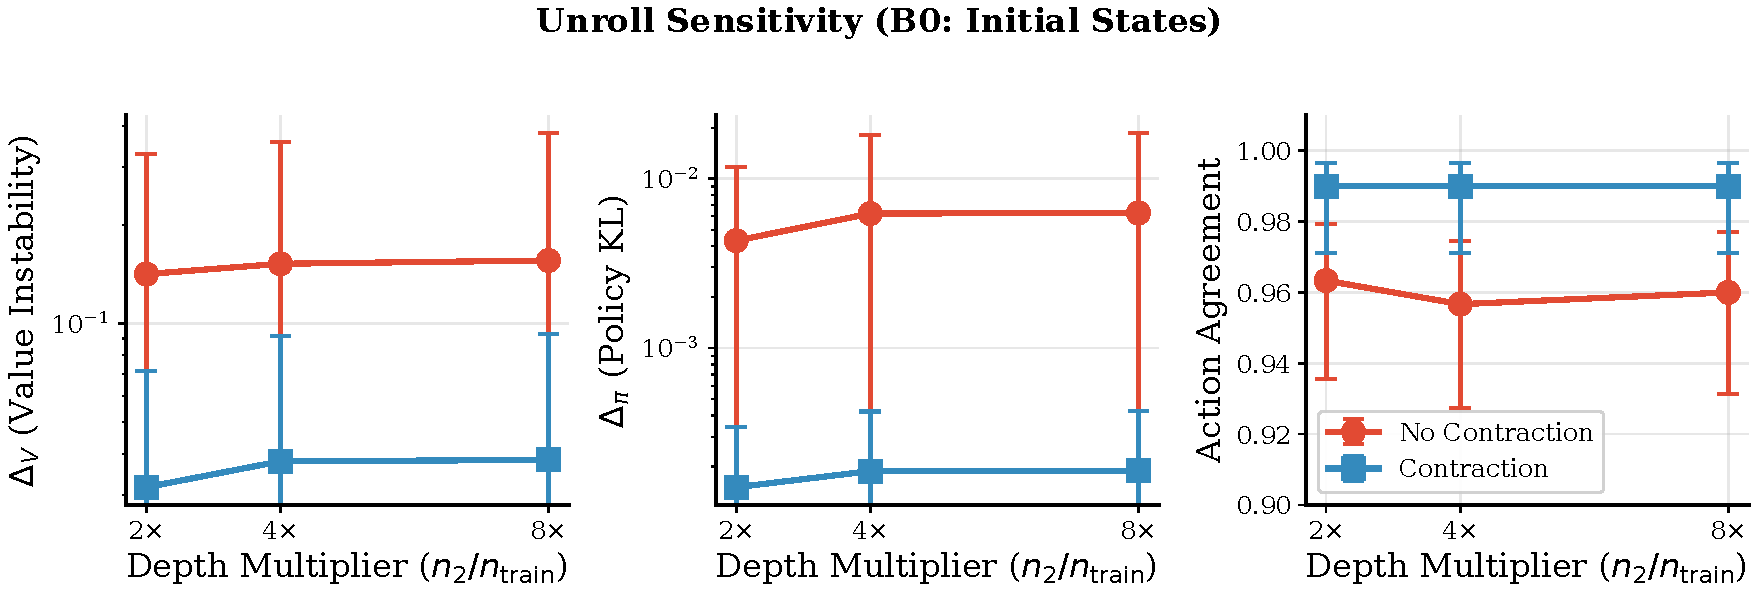
\includegraphics[width=0.75\columnwidth]{figures/fig_exp1_unroll_sensitivity_main.pdf}
\caption{Unroll sensitivity ($n_{\mathrm{train}}{=}2$, $n_{\mathrm{eval}}\in\{4,8,16\}$). Contraction ($L_z{=}0.9$) vs.\ no contraction, $R{=}10$. Contraction reduces drift under depth mismatch.}
\label{fig:exp1_unroll_sensitivity}
\end{figure}

\subsection{Feasibility Results}
\label{sec:feasibility_toy}

On easy 4$\times$4 (1--4 empties, 5k steps, 3 seeds), UPI--TRM achieves $93.3 \pm 2.3\%$ success (no contraction) and $90.7 \pm 5.0\%$ (contraction), vs.\ 52\% random.
On harder 4$\times$4 (6--8 empties, 20k steps, 3 seeds), UPI--TRM reaches 48--57\% while tuned PPO/A2C/DQN (11 configs) achieve \textbf{0\%}.
The modest contraction drop ($90.7$ vs.\ $93.3\%$) reflects the stability/expressivity trade-off.

\begin{table}[t]
\caption{9$\times$9 Sudoku (50k steps, 3 seeds, mean $\pm$ std). All methods use the same TRM backbone and constraint-aware action masking. Score: mean cells correct out of 81; initial puzzle score ${\approx}26.8$. UPI--TRM is the only method that solves any puzzles.}
\label{tab:9x9_results}
\centering
\footnotesize
\setlength{\tabcolsep}{4pt}
\renewcommand{\arraystretch}{0.95}
\begin{tabular}{@{}lccc@{}}
\toprule
Algorithm & Success & Score & Improvement \\
\midrule
\textbf{UPI--TRM} & \textbf{4.0 $\pm$ 4.0\%} & \textbf{53.3 $\pm$ 1.1} & \textbf{+26.5} \\
A2C & 0.0 $\pm$ 0.0\% & 31.9 $\pm$ 0.4 & +5.1 \\
DQN & 0.0 $\pm$ 0.0\% & 29.5 $\pm$ 0.3 & +2.7 \\
PPO & 0.0 $\pm$ 0.0\% & 28.2 $\pm$ 1.5 & +2.2 \\
\bottomrule
\end{tabular}
\end{table}

\textbf{Why do baselines fail on 9$\times$9?}
Standard RL fills a few obvious cells ($+2$ to $+5$) but cannot propagate constraints across the 81-step horizon via a single-pass value estimate.
UPI--TRM's $n$-step latent unroll performs iterative constraint propagation \emph{within each evaluation}; under the contraction condition ($L_z < 1$), the latent iterates converge to a fixed point at rate $L_z^{\,n}$ (Proposition~\ref{prop:banach}), bounding the truncation bias from finite unrolling.
See \Cref{app:9x9_analysis} for a detailed mechanistic analysis.

\subsection{Discussion and Limitations}
\label{sec:discussion}

Two of the three qualitative predictions of the theory are empirically supported (contraction $\to$ less drift, contraction modulus as stability dial); the third ($\alpha$-related) is qualitatively consistent with observed training stability but has not been isolated in a controlled ablation, and several quantities in the bounds ($L_V$, $\varepsilon_{\mathrm{cent}}$, $\varepsilon_{\mathrm{res}}^*$) remain unmeasured.
A detailed mapping is in \Cref{app:theory_practice}.
\textbf{Limitations:}
3 seeds (descriptive);
theory--implementation gaps remain (distillation, centering defect, uncontrolled $L_V$; see \Cref{app:theory_gaps});
experiments restricted to Sudoku (\Cref{app:broader_scope} discusses broader task scope);
projection dominates contraction when both active.
}

\longonly{
\section{Preliminary Experiments}
\label{sec:experiments}
\label{sec:isolation_study}

We report preliminary results on a toy domain to validate that the theoretical dials correlate with empirical behavior.
Comprehensive empirical validation is deferred to future work.

\textbf{Domain: 4$\times$4 Sudoku.}
We use a simplified 4$\times$4 Sudoku with 2$\times$2 blocks.
Let $v(x,y)$ be the number of violated Sudoku \emph{unit constraints} (rows, columns, and $2\times 2$ blocks) for plan $y$ on instance $x$,
where each unit contributes $1$ if it is not a permutation of $\{1,2,3,4\}$
(equivalently, since entries are restricted to $\{1,2,3,4\}$ or blank, the unit contains a repeated digit or an unfilled cell).
There are $4$ rows, $4$ columns, and $4$ blocks, so $0 \le v(x,y) \le 12$.
We define a nonnegative checker score $c(x,y) = C_{\max} - v(x,y)$ with $C_{\max}=12$,
so $c(x,y)=12$ for a valid solution and smaller values indicate more violations.
Edit actions set a single empty cell to a digit in $\{1,2,3,4\}$.

We use $\gamma = 0.99$, $K = 5$, and vary $L_z$ and $n$.


\textbf{Implementation sensitivity of contraction.}
While our theory assumes an $L_z$-contractive latent update map, enforcing this property in practice depends on the chosen norm-control mechanism.
In our implementation, naively applying PyTorch's power-iteration spectral normalization to the inner recursion can be numerically unstable.
We therefore use a simpler and more robust alternative for the $z\!\to\!z$ reasoning layers: explicit operator-norm clamping (rescaling weights when $\|W\|_{\mathrm{op}}$ exceeds a threshold) combined with per-layer output scaling to obtain a strict contraction.
This achieves stable $\hat L_z=O(1)$ in our diagnostics and avoids the numerical blow-ups observed with spectral normalization. Empirically, however, enforcing $L_z<1$ can be overly restrictive and should be treated as a stability/expressivity dial rather than a guarantee of improved success.

\textbf{Correlation between Parameters and Stability.}
We measured the variance of policy updates (gradient norms) and surrogate improvement $\widehat{L}_\pi(\pi_{\mathrm{new}}) - \eta(\pi)$ across training.
Directionally consistent with theory: (i) smaller $L_z$ (stronger contraction) yielded lower gradient variance; (ii) larger $n$ reduced empirical Bellman residuals; (iii) smaller $\alpha$ produced more stable (though slower) improvement.
These observations provide preliminary validation that the theoretical dials translate to practice, though we do not claim tight quantitative agreement.

\begin{figure}[t]
\centering
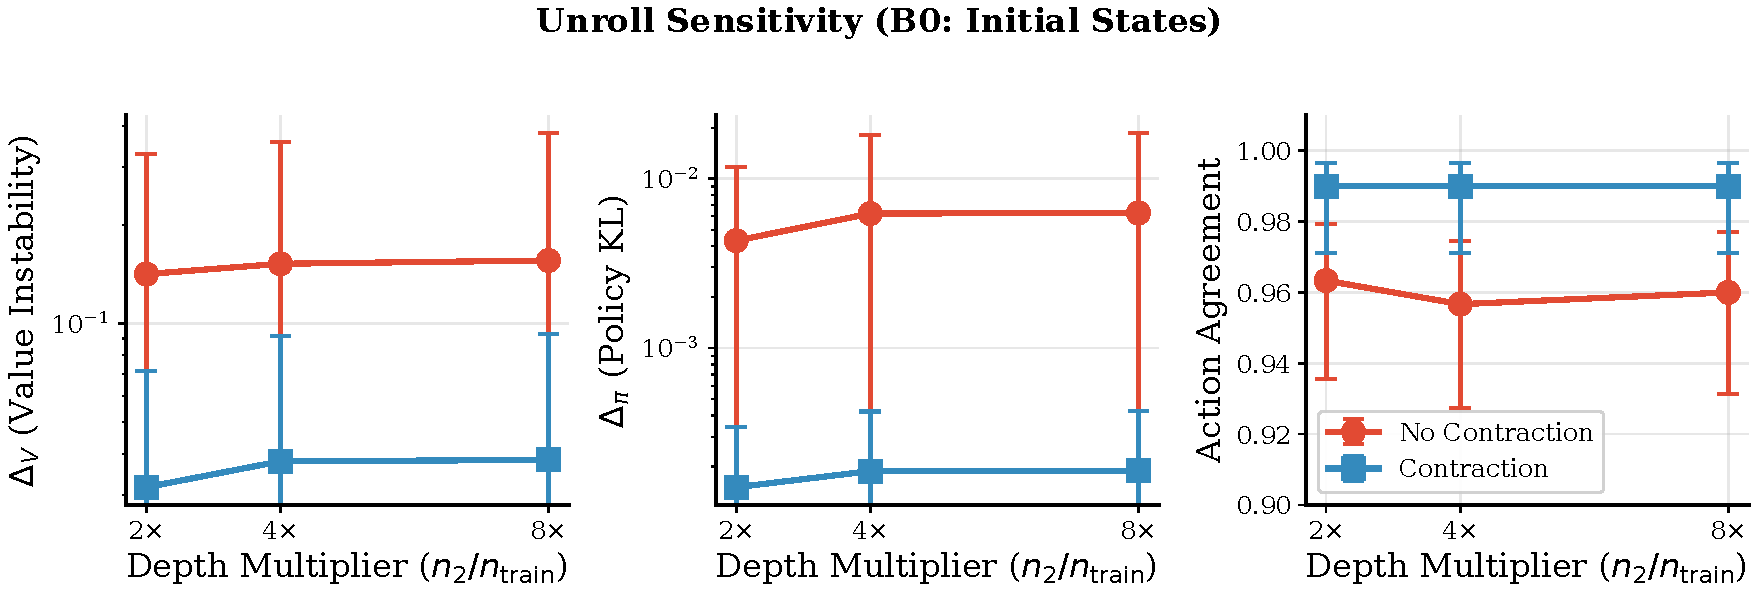
\includegraphics[width=0.88\columnwidth]{figures/fig_exp1_unroll_sensitivity_main.pdf}
\caption{Unroll sensitivity on B0 (initial states). $n_{\mathrm{train}}{=}2$; evaluated at $n_{\mathrm{eval}}\in\{4,8,16\}$ (depth multiplier $n_{\mathrm{eval}}/n_{\mathrm{train}}\in\{2,4,8\}$). ``No Contraction'' vs.\ ``Contraction'' ($L_z{=}0.9$). Both conditions: value-head spectral norm disabled, projection $R{=}10$. Seeds: 41, 42, 43. Left: $\Delta_V$ (value instability, log scale). Center: $\Delta_\pi$ (policy KL, log scale). Right: Argmax Agreement. Error bars: mean$\pm$std ($\Delta_V$, $\Delta_\pi$); Wilson 95\% CI (argmax).}
\label{fig:exp1_unroll_sensitivity}
\end{figure}

\textbf{Completed scale-up: 9$\times$9 Sudoku.}
We scaled UPI--TRM to 9$\times$9 Sudoku (81 cells, 729 actions), a significantly harder domain than 4$\times$4. UPI--TRM shows occasional full solves (4\% episodes) and larger score gains (+26.5) than PPO/A2C/DQN baselines (+2--5 under the same budget). See Section~\ref{sec:9x9_experiments} for details.

\textbf{Proposed additional experiments.}
For future work, we plan:
\begin{itemize}
\item \textbf{Benchmarks:} Maze navigation, ARC-AGI subsets, and other constraint satisfaction tasks.
\item \textbf{Baselines:} (i) Supervised TRM with deep supervision; (ii) ``PPO-on-top'': frozen supervised TRM backbone with PPO on edit policy; (iii) UPI--TRM ablations without contraction enforcement or with $K=1$; (iv) Non-recursive baseline: direct MLP on $(x,y)$ without inner recursion.
\item \textbf{Diagnostics:} Empirical Bellman residuals of $U_n$ on held-out $K$-step rollouts; correlations between unrolled values and Monte Carlo returns; empirical $\hat L_z$, $\hat C_z$, $\widehat{C}_{\mathrm{drift}}(n)$ throughout training; ablation of episodic-$z$ vs.\ persistent-$z$; $\KL(\pi_{\mathrm{new}} \| \pi_\phi)$ after distillation.
\end{itemize}}

\shortonly{
\textbf{Related work.}
TRMs/HRMs~\citep{TRM2025,HRM2025} use iterative refinement; we add RL with checker feedback.
Our plan-space MDP relates to learning-to-search~\citep{Daume2009SEARN,Chang2015LOLS}; contraction analysis connects to DEQs~\citep{Bai2019DEQ}; we build on CPI~\citep{KakadeLangford2002} and RLVR~\citep{Wang2025OneShotRLVR,DeepSeekR1}.}

\longonly{
\section{Related Work}
\label{sec:related_work}

TRM/HRM-style recursive reasoning models~\citep{HRM2025,TRM2025} and follow-ups on training and adaptation~\citep{Qasim2025CGAR,McGovern2025TRMAdapt} motivate our setting.
Our plan-space framing is related to structured prediction as sequential decision making~\citep{Daume2009SEARN,Ross2011DAgger,Chang2015LOLS}, while differing in that we learn from checker rewards rather than expert rollouts.
Our use of automated task checkers also connects to reinforcement learning with verifiable rewards (RLVR), where rewards are computed by verifiers (e.g., exact-match, rule-based checks, or unit tests) rather than learned preference models~\citep{Wang2025OneShotRLVR,Su2025RewardBridge,DeepSeekR1}.
Whereas most RLVR work targets token-level post-training of LLMs, we study verifiable reward in a \emph{plan-editing} MDP and analyze how evaluator design (contraction and finite unrolling) controls evaluation error and conservative improvement.
Model-free RL has also been explored for Sudoku and related deterministic constraint-satisfaction problems, with results indicating poor reliability and weak generalization as difficulty increases~\citep{Mehta2021SudokuRL,Klein2022SudokuRL}.
Technically, we connect contraction of an inner evaluator to approximate dynamic programming error decompositions, contrasting with unrolled DP architectures in environment state space~\citep{Tamar2016VIN,Rozada2025BellNet}.
For safe improvement, we build on conservative policy iteration and trust-region ideas~\citep{KakadeLangford2002,Schulman2015TRPO,Achiam2017CPO}, and we interpret the persistent-$z$ extension through a POMDP-style ``value of memory'' lens~\citep{Kaelbling1998POMDP}.
While Recurrent RL has a long history~\citep{wierstra2007recurrent}, we treat the recurrent state specifically as a computational budget for reasoning, distinct from memory.
Recent work on safe policy iteration~\citep{Pirotta2013SafePI,Metelli2021SafePI} establishes monotonic improvement guarantees under function approximation via constrained optimization formulations; \cite{Eshwar2025MonotoneCPI} extends these ideas beyond the tabular case. Our Theorem~\ref{thm:monotone_with_error} differs in two respects: (i) the $O(\alpha\,\varepsilon_{A,\mathrm{cand}})$ term arises from statewise-centered advantage estimation rather than from trust-region constraints, and (ii) the value decomposition (Proposition~\ref{prop:error_bounds}) explicitly couples policy-improvement to TRM evaluator dials $(L_z, n)$ via the finite-unrolling bias $L_z^n$, bridging architectural design choices to improvement guarantees.

\textbf{Deep equilibrium models.}
Our inner-loop contraction analysis connects to Deep Equilibrium Models~\citep{Bai2019DEQ}, which similarly analyze fixed-point convergence in deep networks, though in a supervised rather than RL setting. Note that the original TRM work emphasizes that fixed-point convergence is not required; our contraction assumption identifies a sufficient (not necessary) regime where theoretical guarantees hold.

\textbf{In-context learning and algorithm distillation.} Algorithm Distillation (AD)~\citep{laskin2022context} trains transformers to emulate RL algorithms by modeling learning histories across episodes, enabling in-context policy improvement without parameter updates. While AD distills a pre-trained RL algorithm (e.g., PPO) into a sequence model, our work analyzes RL training of a recursive evaluator from checker rewards within a single task. Both frameworks treat computation depth (AD: context length; TRM: unroll depth $n$) as a hyperparameter affecting performance; unifying these perspectives---e.g., using TRMs as in-context plan editors---is promising future work.}

\longonly{\textbf{Limitations.}}
\longonly{%
Our analysis uses contraction and Lipschitz assumptions that are only approximately enforced; sup-norm residuals are approximated via $L^2$ losses; guarantees apply to conceptual two-phase GPI with mixtures, not fully interleaved training with distillation.
The persistent-$z$ analysis relies on a slow-drift condition that provides local guidance rather than global guarantees for discrete tasks.
The $O(\alpha \varepsilon_A)$ tightening in Theorem~\ref{thm:monotone_with_error} requires an exactly computed baseline, limiting applicability to discrete action spaces.
Our isolation study (Section~\ref{sec:isolation_study}) provides initial empirical validation: contraction enforcement reduces mismatch drift by $4.1\times$ on value estimates and $33\times$ on policy KL at $8\times$ depth (Figure~\ref{fig:exp1_unroll_sensitivity}).
However, projection at small $R$ can be active 100\%, masking contraction measurements and itself acting as a major stabilizer ($6$--$10\times$ $\Delta_V$ improvement).
Stable training is possible with projection disabled, so projection's role is primarily at evaluation-time mismatch, not training stability.
When projection is disabled, inference-time scaling of the $z\!\to\!z$ recursion yields a measurable range of achieved $L^{\mathrm{pre}}_z$ that correlates monotonically with depth-mismatch stability.
We validated on 9$\times$9 Sudoku (Section~\ref{sec:9x9_experiments}), where UPI--TRM shows occasional solves (4\%) and larger score gains than baselines; further validation on additional domains (e.g., ARC-AGI) remains future work.
Our theoretical bounds use CPI-style conservative mixture updates (mixture weight $\alpha$) as a clean analysis instantiation that yields monotonicity-style statements.
PPO-style clipped objectives are widely used in practice and often more effective, but our current theory does not directly model PPO's implicit trust region via ratio clipping.
Extending the evaluator-error lens to PPO---for instance via KL-regularized surrogate interpretations---is natural future work.
Our experimental validation uses 3 seeds on 4$\times$4 and 9$\times$9 Sudoku; results are descriptive, not statistically significant.
Standard RL baselines (PPO, A2C, DQN) achieved 0\% success on both hard 4$\times$4 (6--8 empties) and 9$\times$9 Sudoku even after hyperparameter tuning, suggesting an advantage of the UPI--TRM design for multi-step constraint satisfaction.}

\longonly{
\textbf{Future directions.}
Comprehensive empirical evaluation on TRM benchmarks; strengthening the POMDP-based analysis; deriving KL trust-region bounds with explicit advantage error; formalizing learned plan embeddings with smoothness regularization; combining with TRM test-time adaptation; and providing rigorous distillation guarantees.}
\bibliography{trm_rl}
\bibliographystyle{iclr2026_conference}

\appendix
\section{Theory--Implementation Gap Details}
\label{app:theory_gaps}

Three quantities in our bounds are not directly measured in current experiments.

\textbf{(a) Distillation gap.}
Theorem~\ref{thm:monotone_with_error} applies to the exact mixture $\pi_{\mathrm{new}}{=}(1{-}\alpha)\pi{+}\alpha\pi_{\mathrm{cand}}$; our implementation distills into a single network $\pi_\phi$.
We monitor $\KL(\pi_{\mathrm{new}} \| \pi_\phi)$ on replay states during training and observe values below $10^{-3}$ throughout, suggesting the distillation gap is small relative to the improvement signal.
By Pinsker's inequality, this implies per-state total-variation distance below $0.03$.
\emph{Caveat:} this measurement uses replay-buffer states, not a held-out set.
Because our replay buffer is refreshed each iteration with on-policy rollouts and covers all reachable states in the small 4$\times$4 domain, replay-state KL is a reasonable proxy for held-out KL; confirming this on a separate held-out partition is planned.
A formal distillation-gap bound (e.g., via $\eta(\pi_{\mathrm{new}}) - \eta(\pi_\phi) \le \tfrac{2\gamma}{(1-\gamma)^2}\sup_s \|\pi_{\mathrm{new}}(\cdot|s) - \pi_\phi(\cdot|s)\|_{\mathrm{TV}}$) remains future work.

\textbf{(b) Centering defect.}
Our experiments use GAE-style baselines, providing approximate rather than exact statewise centering.
The centering defect is defined as $\varepsilon_{\mathrm{cent}} := \sup_s |\sum_a \pi(a|s)\,\widehat{A}(s,a)|$; for discrete action spaces this is directly computable by enumerating actions at each state in a held-out batch.
We expect $\varepsilon_{\mathrm{cent}}$ to be small in our setting for three reasons: the action space is discrete and moderate-sized (97 actions for 4$\times$4, 729 for 9$\times$9), the baseline $B_V(s) = \E_{b\sim\pi}[\widehat{Q}_V(s,b)]$ is computed by full summation over valid actions (not sampled), and the policy is near-converged at evaluation time.
We leave empirical measurement of $\varepsilon_{\mathrm{cent}}$ to future work.
With nonzero $\varepsilon_{\mathrm{cent}}$, the bound degrades to $O(\alpha\varepsilon_{A,\mathrm{cand}} + \varepsilon_{\mathrm{cent}})$ rather than $O(\alpha\varepsilon_{A,\mathrm{cand}})$; the factors above suggest this degradation is modest, but quantifying it is a concrete open item.

\textbf{(c) Value-head Lipschitz constant $L_V$.}
We disable value-head spectral normalization to avoid training instability, so $L_V$ in Eq.~\eqref{eq:epsV_dials} is uncontrolled during training.
The value-head is a 2-layer MLP without explicit norm constraints; we do not measure its spectral norm post-hoc in the current experiments.
This means the bound in Eq.~\eqref{eq:epsV_dials} provides qualitative structural guidance (identifying which quantities matter) rather than a quantitative guarantee.
Measuring and reporting $L_V$ across training checkpoints is a concrete diagnostic we leave to future work.

\section{Experiment Setup Details}
\label{app:exp_setup}

\textbf{4$\times$4 Sudoku:} horizon $T{=}16$, $\gamma{=}0.99$, 97 actions with state-dependent masking.
Contraction ($L_z{=}0.9$) enforced via operator-norm clamping on $z\!\to\!z$ layers; projection $\Pi_R$ onto radius-$R$ ball.
Value-head spectral normalization disabled in all stability experiments.
Episodic-$z$ mode (latent reinitialized each edit step); shaped reward as in Section~\ref{sec:setup}.
All networks are 2-layer MLPs ($d{=}128$); $\pi_\phi$ uses masked softmax.
Adam optimizer, LR $3{\times}10^{-4}$; PPO clip $\epsilon{=}0.2$, entropy coefficient $0.01$.
Step budgets refer to environment steps (each step = one edit action).

\textbf{9$\times$9 Sudoku:} 81 cells, 729 actions (81 positions $\times$ 9 digits), constraint-aware masking reduces to ${\sim}250$ valid actions per state.
Horizon $T{=}81$, $\gamma{=}0.99$, 50k training steps, 3 seeds.
Score: filled cells $- 2.0 \times$ violations $- 5.0 \times$ zero-candidate cells; initial puzzle score ${\approx}26.8$, maximum 81.

\section{Theory--Practice Bridge}
\label{app:theory_practice}

Our theoretical bounds make qualitative predictions that map to experimental observations:
\begin{enumerate}[nosep,leftmargin=*]
\item \emph{Stronger contraction $\to$ less drift under depth mismatch} (Proposition~\ref{prop:error_bounds}, $L_z^{\,n}$ term): empirically supported---contraction reduces $\Delta_V$ by $4.1\times$ and $\Delta_\pi$ by $33\times$ at $8\times$ depth mismatch (\Cref{fig:exp1_unroll_sensitivity}).
\item \emph{Contraction modulus as stability dial}: supported when projection is disabled---$L_z^{\mathrm{pre}}$ correlates monotonically with depth-mismatch stability (Pearson $\rho = -0.87$ on initial states).
\item \emph{Conservative $\alpha$ limits sensitivity to evaluation error} (Theorem~\ref{thm:monotone_with_error}): qualitatively consistent with stable training, though $\alpha$ has not been isolated in a controlled ablation.
\end{enumerate}
Full quantitative validation of Eq.~\eqref{eq:epsV_dials} requires measuring $L_V$, $\varepsilon_{\mathrm{res}}^*$, and $\varepsilon_{\mathrm{cent}}$; the centering defect is expected to be small (discrete actions, exact baseline summation; see \Cref{app:theory_gaps}).

\section{9$\times$9 Sudoku: Mechanistic Analysis}
\label{app:9x9_analysis}

Standard RL methods (PPO, A2C, DQN) learn to fill a few obvious cells (score improvements of $+2$ to $+5$) but cannot propagate constraint information across the 81-step edit horizon needed to complete the puzzle---they rely on a single forward pass for value estimation, which is insufficient for the combinatorial credit assignment required by 9$\times$9 Sudoku.
UPI--TRM's recursive evaluator provides a structural advantage: the $n$-step latent unroll performs iterative internal computation \emph{within each evaluation}, enabling multi-step constraint propagation that a single forward pass cannot achieve.
Under the contraction condition ($L_z < 1$), the latent iterates converge to a fixed point at rate $L_z^{\,n}$ (Proposition~\ref{prop:banach}), bounding the truncation bias introduced by finite unrolling; the Bellman-residual term in Proposition~\ref{prop:error_bounds} captures how well the converged architecture approximates long-horizon value.
Note that the current experiments use \emph{episodic-$z$} (the latent is reinitialized at each edit step); a persistent-$z$ extension that carries the latent across steps is an untested direction sketched in Section~\ref{sec:setup}.
Flat baselines lack this iterative internal computation altogether.

\section{Broader Task Scope}
\label{app:broader_scope}

Our experiments are restricted to Sudoku, a controlled constraint-satisfaction domain.
The theoretical results apply to any architecture meeting the contraction assumptions (Remark~\ref{rem:generality}), but empirical generality remains unvalidated.
Testing generality requires domains with qualitatively different structure:
\begin{itemize}[nosep,leftmargin=*]
\item \emph{Maze navigation:} sparse terminal reward, longer horizons ($T \gg 16$)---stresses the $K$-step bootstrap and discount sensitivity. The contraction dial would need to balance expressivity against stability over many more edit steps.
\item \emph{ARC-AGI subsets:} variable grid sizes, abstract pattern rules---challenges action-space scaling and out-of-distribution generalization of the learned evaluator. The inner recursion must generalize across structurally diverse inputs.
\item \emph{Code repair with unit tests:} large discrete action space, binary pass/fail reward---probes whether checker feedback scales beyond constraint satisfaction to domains with sparser and more delayed reward signals.
\end{itemize}
A meaningful positive result would show that the contraction/unroll-depth dials transfer: stronger contraction reduces depth-mismatch drift in the new domain.
A meaningful negative result would identify regimes where contraction is too restrictive to permit learning, bounding the applicability of our analysis and motivating relaxations (e.g., local contraction or adaptive $L_z$ schedules).

\shortonly{
\section{Deferred Technical Results}
\label{app:deferred}

\textbf{Persistent-$z$ (sketch).}
The original TRM carries the latent across edits.
We extend bounds under a slow-drift assumption on the moving fixed point $z^*(x,y_t)$: value/advantage error has the same form as the episodic-$z$ case, but with $L_z^n C_z/(1{-}L_z)$ replaced by a drift term $C_{\mathrm{drift}}(n)$ capturing tracking error of the moving fixed point.
Persistent-$z$ variants reuse computation but incur an additional ``value-of-memory'' / tracking penalty when history matters.
}

\end{document}
